%% Beamer-Klasse im korrekten Modus
\documentclass{beamer}
\usepackage{subcaption}
%\documentclass[18pt,parskip]{beamer}

%% SLIDE FORMAT

% use 'beamerthemekit' for standard 4:3 ratio
% for widescreen slides (16:9), use 'beamerthemekitwide'

\usepackage{../templates/KIT-slides/beamerthemekitwide}
%\usepackage{../templates/KIT-slides/beamerthemekitwide}

%% TITLE PICTURE

% if a custom picture is to be used on the title page, copy it into the 'logos'
% directory, in the line below, replace 'mypicture' with the 
% filename (without extension) and uncomment the following line
% (picture proportions: 63 : 20 for standard, 169 : 40 for wide
% *.eps format if you use latex+dvips+ps2pdf, 
% *.jpg/*.png/*.pdf if you use pdflatex)

\titleimage{../figures/titleimage/brain}

%% TITLE LOGO

% for a custom logo on the front page, copy your file into the 'logos'
% directory, insert the filename in the line below and uncomment it

\newcommand{\titlelogo}{../../media/logoHQ.png}
%\titlelogo{../media/logoHQ.png}

% (*.eps format if you use latex+dvips+ps2pdf,
% *.jpg/*.png/*.pdf if you use pdflatex)

%% TikZ INTEGRATION

% use these packages for PCM symbols and UML classes
% \usepackage{templates/tikzkit}
% \usepackage{templates/tikzuml}

%\usepackage{tikz}
%\usetikzlibrary{matrix}
%\usetikzlibrary{arrows.meta}
%\usetikzlibrary{automata}
%\usetikzlibrary{tikzmark}

%%%%%%%%%%%%%%%%%%%%%%%%%
% Libertine font (Original GBI font)
\usepackage[mono=false]{libertine}
%\renewcommand*\familydefault{\sfdefault}  %% Only if the base font of the document is to be sans serif

%% Schönere Schriften
\usepackage[TS1,T1]{fontenc}

%% Deutsche Silbentrennung und Beschriftungen
\usepackage[ngerman]{babel}

%% UTF-8-Encoding
\usepackage[utf8]{inputenc}

%% Bibliotheken für viele mathematische Symbole
\usepackage{amsmath, amsfonts, amssymb}

%% Anzeigetiefe für Inhaltsverzeichnis: 1 Stufe
\setcounter{tocdepth}{1}

%% Hyperlinks
\usepackage{hyperref}
% I don't know why, but this works and only includes sections and NOT subsections in the pdf-bookmarks.
\hypersetup{bookmarksdepth=subsection}

%% remove navigation symbols
\setbeamertemplate{navigation symbols}{}

%% switch between "ngerman" and "english" for German/English style date and logos
\selectlanguage{ngerman}

\usepackage{xcolor}

%% for invisible pause texts instead of dimming
\setbeamercovered{invisible}

\usepackage[german=swiss]{csquotes}

\usepackage{tabularx}
\usepackage{booktabs}

%\usepackage{tikz}
%\usetikzlibrary{arrows,automata,positioning}

\usepackage{xspace}

\usepackage{graphicx}

\usepackage{verbatim}

\usepackage{algorithm}
\usepackage[]{algpseudocode}
\algrenewcommand{\algorithmiccomment}[1]{\hfill\(//\) #1}

\usepackage[outdir=./]{epstopdf}

% Problem: disabled itemize-icons
%\usepackage{enumitem}
% %\setlist[enumerate]{topsep=0pt,itemsep=-1ex,partopsep=1ex,parsep=1ex}
% \setlist[itemize]{noitemsep, nolistsep}
% \setlist[enumerate]{noitemsep, nolistsep}


\AtBeginDocument{
\abovedisplayskip=0pt
\belowdisplayskip=0pt
\abovedisplayshortskip=0pt
\belowdisplayshortskip=0pt
}
%%%%%%%%%%%% Slides %%%%%%%%%%%%%%%%

%% Titelinformationen
\author{Katharina Biernacka \and Maria Kraus \and Fabian Reinbold \and Daniel Schild}
\institute{Fakultät für Informatik}
%\date{\mydate}

%% Titel einfügen
\newcommand{\titleframe}{\frame{\titlepage}\addtocounter{framenumber}{-1}}

%% Emph be queen
\setbeamercolor{emph}{fg=kit-green100}
\renewcommand<>{\emph}[1]{%
  {\usebeamercolor[fg]{emph}\only#2%{\itshape}
  #1}%
}

%% Roadmap frame
%table of contents
\newcommand{\roadmap}{
	\frame{\frametitle{Roadmap}\tableofcontents}}

 \AtBeginSection[]{%
\begin{frame}
	\frametitle{Roadmap}
	\tableofcontents[currentsection]
\end{frame}%\addtocounter{framenumber}{-1}
}


%% ShowMessage frame
\newcommand{\showmessage}[1]{\frame{\frametitle{\phantom{1em}}\centering\textbf{#1}}}

%% Fragen
\newcommand{\questionframe}{\showmessage{Fragen?}}

%% Lastframe
\newcommand{\lastframe}{\showmessage{Vielen Dank für Ihre Aufmerksamkeit!}}

\newcommand{\softwarename}{VisAQ }
\newcommand{\longSoftwarename}{Visualizing Air Quality}

% Allgemein
\renewcommand{\gets}{\ensuremath{\leftarrow}}
\newcommand{\Rplus}{\ensuremath{\nR_+}}
\newcommand{\Rnullplus}{\ensuremath{\nR^+_0}}
\newcolumntype{C}{>{$}c<{$}} % math-mode version of "C" column type

% O Kalkül
\newcommand{\Oh}{\ensuremath{\mathcal{O}}}

% Pseudocode
\renewcommand{\:}{$\; : \;$}
\newcommand{\newpar}[1]{\paragraph{#1}\mbox{}\newline}

\newcommand{\nM}{\mathbb{M}}
\newcommand{\nR}{\mathbb{R}}
\newcommand{\nN}{\mathbb{N}}
\newcommand{\nZ}{\mathbb{Z}}
\newcommand{\nQ}{\mathbb{Q}}
\newcommand{\nB}{\mathbb{B}}
\newcommand{\nC}{\mathbb{C}}
\newcommand{\nK}{\mathbb{K}}
\newcommand{\nF}{\mathbb{F}}
\newcommand{\nG}{\mathbb{G}}
\newcommand{\nullel}{\mathcal{O}}
\newcommand{\einsel}{\mathds{1}}
\newcommand{\nP}{\mathbb{P}}
\newcommand{\Pot}{\mathcal{P}}
%\renewcommand{\O}{\text{O}}

\newcommand{\bfmod}{\ensuremath{\text{\textbf{ mod }}}}
\renewcommand{\mod}{\bfmod}
\newcommand{\bfdiv}{\ensuremath{\text{\textbf{ div }}}}
\renewcommand{\div}{\bfdiv}


\newcommand{\set}[1]{\left\{ #1 \right\}}
\newcommand{\setc}[2]{\set{#1 \mid #2}}
\newcommand{\setC}[2]{\set{#1 \mid \text{ #2 }}}

\newcommand{\setsize}[1]{\; \mid #1 \mid \; }

\newcommand{\q}[1]{\textquotedblleft #1\textquotedblright}

% Zu zeigen, thx to http://www.matheboard.de/archive/155832/thread.html
\newcommand{\zz}{\ensuremath{\mathrm{z\kern-.29em\raise-0.44ex\hbox{z}}}:}

% Text above symbol
% https://tex.stackexchange.com/a/74132/146825
%
% \newcommand{\eqtext}[1]{\stackrel{\mathclap{\normalfont\mbox{#1}}}{=}}
% \newcommand{\gdwtext}[1]{\stackrel{\mathclap{\normalfont\mbox{#1}}}{\Leftrightarrow}}
% \newcommand{\imptext}[1]{\stackrel{\mathclap{\normalfont\mbox{#1}}}{\Rightarrow}}
% \newcommand{\symbtext}[2]{\stackrel{\mathclap{\normalfont\mbox{#2}}}{#1}}
\newcommand{\eqtext}[1]{\mathrel{\overset{\makebox%[0pt]
{\mbox{\normalfont\tiny #1}}}{=}}}
\newcommand{\gdwtext}[1]{\mathrel{\overset{\makebox%[0pt]
{\mbox{\normalfont\tiny #1}}}{\ensuremath{\Leftrightarrow}}}}
\newcommand{\imptext}[1]{\mathrel{\overset{\makebox%[0pt]
{\mbox{\normalfont\tiny #1}}}{\ensuremath{\Rightarrow}}}}
\newcommand{\symbtext}[2]{\mathrel{\overset{\makebox%[0pt]
{\mbox{\normalfont\tiny #2}}}{#1}}}

% qed symbol
\newcommand{\qedblack}{\hfill \ensuremath{\blacksquare}}
\newcommand{\qedwhite}{\hfill \ensuremath{\Box}}

% Aussagenlogik
% Worsch
\colorlet{alcolor}{blue}
\RequirePackage{tikz}
\usetikzlibrary{arrows.meta}
\newcommand{\alimpl}{\mathrel{\tikz[x={(0.1ex,0ex)},y={(0ex,0.1ex)},>={Classical TikZ Rightarrow[]}]{\draw[alcolor,->,line width=0.7pt,line cap=round] (0,0) -- (15,0);\path (0,-6);}}}
\newcommand{\alimp}{\alimpl}
\newcommand{\aleqv}{\mathrel{\tikz[x={(0.1ex,0ex)},y={(0ex,0.1ex)},>={Classical TikZ Rightarrow[]}]{\draw[alcolor,<->,line width=0.7pt,line cap=round] (0,0) -- (18,0);\path (0,-6);}}}
\newcommand{\aland}{\mathbin{\raisebox{-0.6pt}{\rotatebox{90}{\texttt{\color{alcolor}\char62}}}}}
\newcommand{\alor}{\mathbin{\raisebox{-0.8pt}{\rotatebox{90}{\texttt{\color{alcolor}\char60}}}}}
%\newcommand{\ali}[1]{_{\mathtt{\color{alcolor}#1}}}
\newcommand{\alv}[1]{\mathtt{\color{alcolor}#1}}
\newcommand{\alnot}{\mathop{\tikz[x={(0.1ex,0ex)},y={(0ex,0.1ex)}]{\draw[alcolor,line width=0.7pt,line cap=round,line join=round] (0,0) -- (10,0) -- (10,-4);\path (0,-8) ;}}}
\newcommand{\alP}{\alv{P}} %ali{#1}}
%\newcommand{\alka}{\negthinspace\hbox{\texttt{\color{alcolor}(}}}
\newcommand{\alka}{\negthinspace\text{\texttt{\color{alcolor}(}}}
%\newcommand{\alkz}{\texttt{\color{alcolor})}}\negthinspace}
\newcommand{\alkz}{\text{\texttt{\color{alcolor})}}\negthinspace}

% Thassilo
\newcommand{\BB}{\mathbb{B}}
\newcommand{\boder}{\alor}%{\ensuremath{\text{\;}\textcolor{blue}{\vee}}\text{\;}}
\newcommand{\bund}{\aland}%{\ensuremath{\text{\;}\textcolor{blue}{\wedge}}\text{\;}}
\newcommand{\bimp}{\alimp}%{\ensuremath{\text{\;}\textcolor{blue}{\to}}\text{\;}}
\newcommand{\bnot}{\alnot}%{\ensuremath{\text{\;}\textcolor{blue}{\neg}}\text{}}
\newcommand{\bgdw}{\aleqv}%{\ensuremath{\text{\;}\textcolor{blue}{\leftrightarrow}}\text{\;}}
\newcommand{\bone}{\ensuremath{\textcolor{blue}{1}}\text{}}
\newcommand{\bzero}{\ensuremath{\textcolor{blue}{0}}\text{}}
\newcommand{\bleftBr}{\alka}%{\ensuremath{\textcolor{blue}{(}}\text{}}
\newcommand{\brightBr}{\alkz}%{\ensuremath{\textcolor{blue}{)}}\text{}}

\newcommand{\val}{\hbox{\textit{val}}}

\newcommand{\VarAL}{\hbox{\textit{Var}}_{AL}}
\newcommand{\ForAL}{\hbox{\textit{For}}_{AL}}

% Validierungsfunktion val_i
\newcommand{\vali}[1]{\ensuremath{\val_I(#1)}}

% Boolsche Funktion b_
\newcommand{\bfnot}[1]{\ensuremath{b_{\bnot}(#1)}}
\newcommand{\bfand}[2]{\ensuremath{b_{\bund}(#1,#2)}}
\newcommand{\bfor}[2]{\ensuremath{b_{\boder}(#1,#2)}}
\newcommand{\bfimp}[2]{\ensuremath{b_{\bimp}(#1,#2)}}

% Aussagenkalkül
\newcommand{\AAL}{A_{AL}}
\newcommand{\LAL}{\hbox{\textit{For}}_{AL}}
\newcommand{\AxAL}{\hbox{\textit{Ax}}_{AL}}
\newcommand{\MP}{\hbox{\textit{MP}}}

% Prädikatenlogik
% die nachfolgenden Sachen angepasst an cmtt
\newlength{\ttquantwd}
\setlength{\ttquantwd}{1ex}
\newlength{\ttquantht}
\setlength{\ttquantht}{6.75pt}
\def\plall{%
  \tikz[line width=0.67pt,line cap=round,line join=round,baseline=(B),alcolor] {
    \draw (-0.5\ttquantwd,\ttquantht) -- node[coordinate,pos=0.4] (lll){} (-0.25pt,-0.0pt) -- (0.25pt,-0.0pt) -- node[coordinate,pos=0.6] (rrr){} (0.5\ttquantwd,\ttquantht);
    \draw (lll) -- (rrr);
    \coordinate (B) at (0,-0.35pt);
  }%
}
\def\plexist{%
  \tikz[line width=0.67pt,line cap=round,line join=round,baseline=(B),alcolor] {
    \draw (-0.9\ttquantwd,\ttquantht) -- (0,\ttquantht) -- node[coordinate,pos=0.5] (mmm){} (0,0) --  (-0.9\ttquantwd,0);
    \draw (mmm) -- ++(-0.75\ttquantwd,0);
    \coordinate (B) at (0,-0.35pt);
  }\ensuremath{\,}%
}
\let\plexists=\plexist
\newcommand{\NT}[1]{\ensuremath{\langle\mathrm{#1} \rangle}}
\newcommand{\CPL}{\text{\itshape Const}_{PL}}
\newcommand{\FPL}{\text{\itshape Fun}_{PL}}
\newcommand{\RPL}{\text{\itshape Rel}_{PL}}
\newcommand{\VPL}{\text{\itshape Var}_{PL}}
\newcommand{\plka}{\alka}
\newcommand{\plkz}{\alkz}
%\newcommand{\plka}{\plfoo{(}}
%\newcommand{\plkz}{\plfoo{)}}
\newcommand{\plcomma}{\hbox{\texttt{\color{alcolor},}}}
\newcommand{\pleq}{{\color{alcolor}\,\dot=\,}}

\newcommand{\plfoo}[1]{\mathtt{\color{alcolor}#1}}
\newcommand{\plc}{\plfoo{c}}
\newcommand{\pld}{\plfoo{d}}
\newcommand{\plf}{\plfoo{f}}
\newcommand{\plg}{\plfoo{g}}
\newcommand{\plh}{\plfoo{h}}
\newcommand{\plx}{\plfoo{x}}
\newcommand{\ply}{\plfoo{y}}
\newcommand{\plz}{\plfoo{z}}
\newcommand{\plR}{\plfoo{R}}
\newcommand{\plS}{\plfoo{S}}
\newcommand{\ar}{\mathrm{ar}}

\newcommand{\bv}{\mathrm{bv}}
\newcommand{\fv}{\mathrm{fv}}

\def\word#1{\hbox{\textcolor{blue}{\texttt{#1}}}}
%\let\literal\word
\def\mword#1{\hbox{\textcolor{blue}{$\mathtt{#1}$}}}  % math word
\def\sp{\scalebox{1}[.5]{\textvisiblespace}}
\def\wordsp{\word{\sp}}


\newcommand{\W}{\ensuremath{\hbox{\textbf{w}}}\xspace}
\newcommand{\F}{\ensuremath{\hbox{\textbf{f}}}\xspace}
\newcommand{\WF}{\ensuremath{\{\W,\F\}}\xspace}
\newcommand{\valDIb}{\val_{D,I,\beta}}

\newcommand{\impl}{\ifmmode\ensuremath{\mskip\thinmuskip\Rightarrow\mskip\thinmuskip}\else$\Rightarrow$\fi\xspace}
\newcommand{\Impl}{\ifmmode\implies\else$\Longrightarrow$\fi\xspace}

\newcommand{\derives}{\Rightarrow}

\newcommand{\gdw}{\ifmmode\mskip\thickmuskip\Leftrightarrow\mskip\thickmuskip\else$\Leftrightarrow$\fi\xspace}
\newcommand{\Gdw}{\ifmmode\iff\else$\Longleftrightarrow$\fi\xspace}

\newcommand*{\from}{\colon}
\newcommand{\functionto}{\longrightarrow}


\newcommand{\LTer}{L_{\text{\itshape Ter}}}
\newcommand{\LRel}{L_{\text{\itshape Rel}}}
\newcommand{\LFor}{L_{\text{\itshape For}}}
\newcommand{\NTer}{N_{\text{\itshape Ter}}}
\newcommand{\NRel}{N_{\text{\itshape Rel}}}
\newcommand{\NFor}{N_{\text{\itshape For}}}
\newcommand{\PTer}{P_{\text{\itshape Ter}}}
\newcommand{\PRel}{P_{\text{\itshape Rel}}}
\newcommand{\PFor}{P_{\text{\itshape For}}}

\newcommand{\sgn}{\mathop{\text{sgn}}}

\newcommand{\lang}[1]{\ensuremath{\langle#1\rangle}}

\newcommand{\literal}[1]{\hbox{\textcolor{blue!95!white}{\textup{\texttt{\scalebox{1.11}{#1}}}}}}
\let\hashtag\#
\renewcommand{\#}[1]{\literal{#1}}

\def\blank{\ensuremath{\openbox}}
\def\9{\blank}
\newcommand{\io}{\!\mid\!}


\providecommand{\fspace}{\mathord{\text{space}}}
\providecommand{\fSpace}{\mathord{\text{Space}}}
\providecommand{\ftime}{\mathord{\text{time}}}
\providecommand{\fTime}{\mathord{\text{Time}}}

\newcommand{\fnum}{\text{num}}
\newcommand{\fNum}{{\text{Num}}}

\def\Pclass{\text{\bfseries P}}
\def\PSPACE{\text{\bfseries PSPACE}}

\title{PSE 2020 \textbf{VisAQ}}
\subtitle{Anwenderorientierte Nutzerschnittstelle für Luftqualitätsdaten Team 2}
\date{\today}

\usetikzlibrary{matrix}
\usetikzlibrary{arrows.meta}
\usetikzlibrary{automata}
\usetikzlibrary{tikzmark}
\usetikzlibrary{arrows}
\usetikzlibrary{positioning}
\usetikzlibrary{quotes}

\usetikzlibrary{shapes}

\begin{document}
\titleframe


\roadmap

\section{VisAQ: Unsere Leistungen im Überblick}
\begin{frame}{VisAQ - Visualizing Air Quality}
    Ziel ist die Entwicklung einer Anwenderorientierte Nutzerschnittstelle für Luftqualitätsdaten
\end{frame}
\begin{frame}{Nutzerstudie}
    Ermittelt Nutzerverhalten und Bedürfnisse
\end{frame}
\begin{frame}{Nutzerstudie - Altersverteilung}
    \begin{figure}[h]
        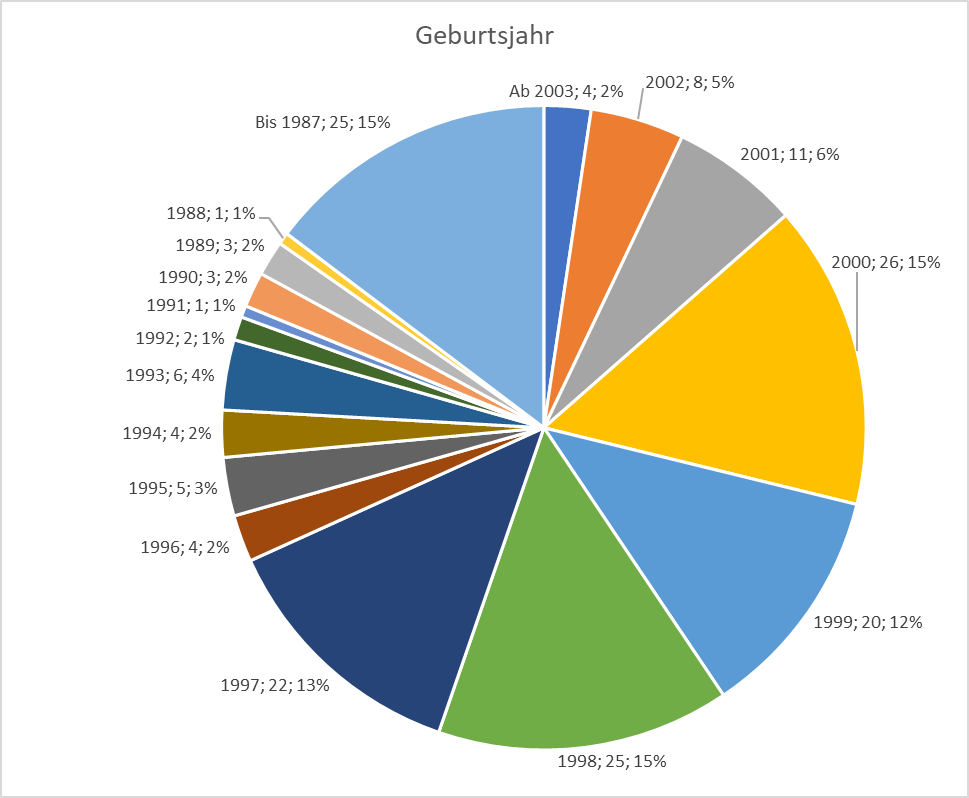
\includegraphics[height=0.7\textheight]{../../media/diagram/geburtsjahr}
    \end{figure}
\end{frame}
\begin{frame}{Nutzerstudie - Selbsteinschätzung}
    \begin{figure}[h]
        \begin{subfigure}[c]{0.49\textwidth}
            \centering        
            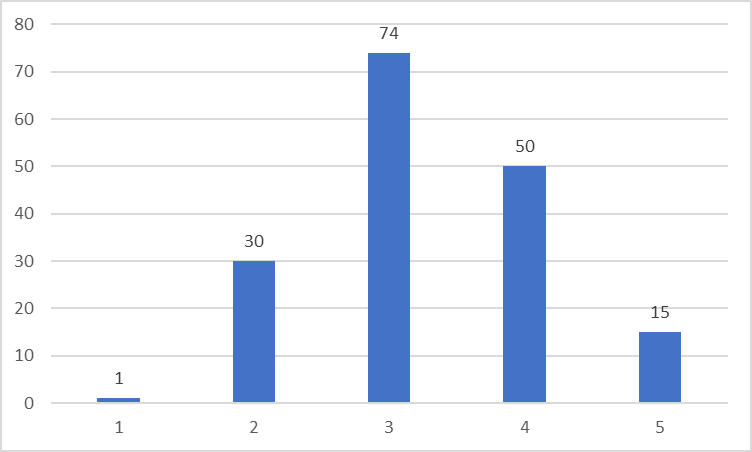
\includegraphics[scale=0.2]{../../media/diagram/eigenesWissen.png}
            \subcaption{Einschätzung zum eigenen Wissen über Luftverschmutzung}
        \end{subfigure}
        \begin{subfigure}[c]{0.49\textwidth}
            \centering        
            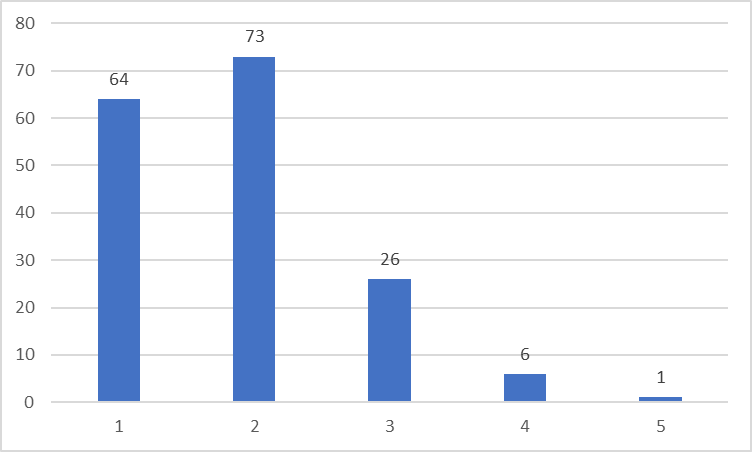
\includegraphics[scale=0.2]{../../media/diagram/WichtigkeitVonInfos.png}
            \subcaption{Einschätzung zur Wichtigkeit von Informationen über Luftverschmutzung}
        \end{subfigure}
    \end{figure}
\end{frame}
\begin{frame}{Nutzerstudie - Aufrufshäufigkeit}
    \begin{figure}[h]
        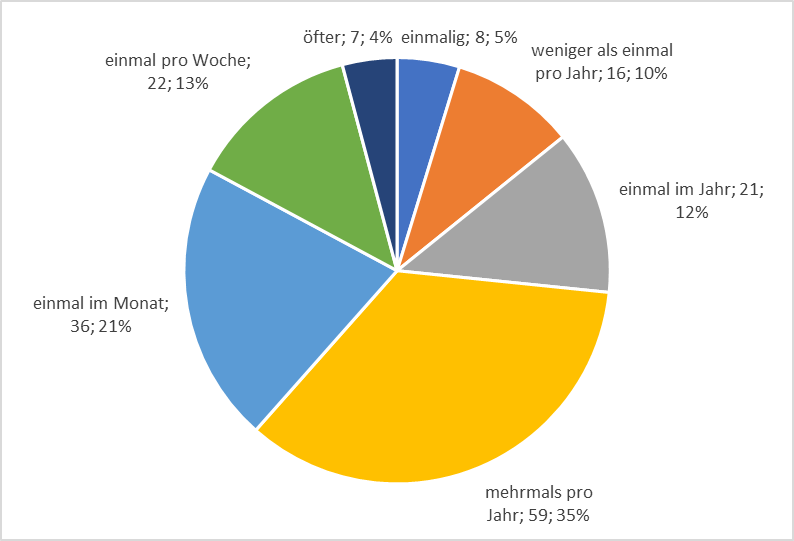
\includegraphics[height=0.7\textheight]{../../media/diagram/aufrufe}
    \end{figure}
\end{frame}
\begin{frame}{Nutzerstudie - Informationsbedürfniss}
    \begin{figure}[h]
        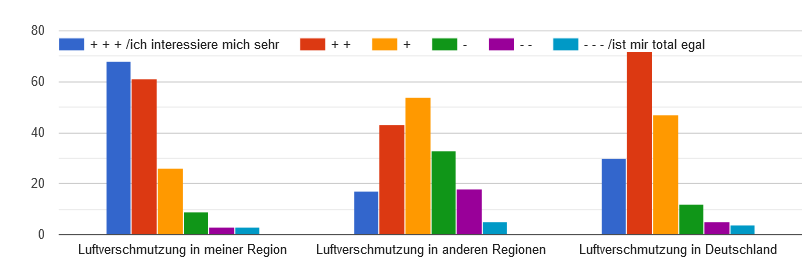
\includegraphics[height=0.35\textheight]{../../media/diagram/interesse}
    \end{figure}
    \begin{figure}[h]
        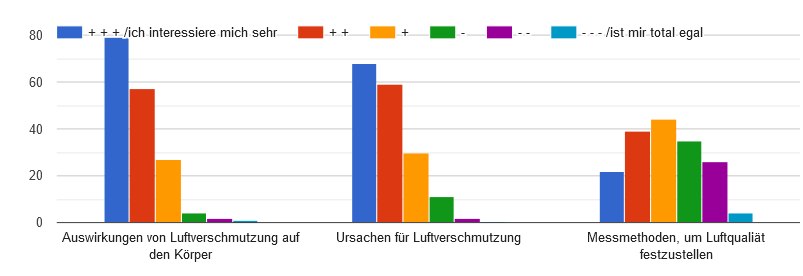
\includegraphics[height=0.35\textheight]{../../media/diagram/interesse2}
    \end{figure}
\end{frame}
\begin{frame}{Nutzerstudie - Sonstige Ergebnisse}
    \centering
    Nutzergeräte
    \\
    \vspace{1cm}
    Allgemeine Anregungen
\end{frame}
\section{Der Aufbau des Systems}
\begin{frame}{Systemmodell}
    \begin{figure} [h]
        \scalebox{.75}{
            \begin{tikzpicture}[node distance=2cm]
        
                %Model
                \begin{scope}[shift={(0,0)},local bounding box=M]
                    \draw (0,0) [dashed] rectangle (4.5,6);
                    \node[scale=1] at (2.25,5.5) {Model};
                    \begin{scope}[local bounding box=Datenbank]
                        \draw (0.25,2.5) rectangle (4.25,4.5);
                        \node[scale=0.8] at (2.25,3.5) {SensorThings Datenbank};
                    \end{scope}
                    \begin{scope}[local bounding box=Sensoren]
                        \draw (0.25,0.5) rectangle (4.25,1.5);
                        \node[scale=0.8] at (2.25,1) {Heterogenes Sensor-Netz};
                    \end{scope}
                \end{scope}
                
                %Controller
                \begin{scope}[shift={(5.25,0)},local bounding box=C]
                    \draw (0,0) [dashed] rectangle (4.5,6);
                    \node[scale=1] at (2.25,5.5) {Controller};
                    \begin{scope}[local bounding box=Backend]
                        \draw (0.25,2.5) rectangle (4.25,4.5);
                        \node[scale=0.8] at (2.25,3.5) {\softwarename Backend};
                    \end{scope}
                    \begin{scope}[local bounding box=User-Backend]
                        \draw (0.25,0.5) rectangle (4.25,1.5);
                        \node[scale=0.8] at (2.25,1) {Java-Script Controller};
                    \end{scope}
                \end{scope}
        
                %View
                \begin{scope}[shift={(10.5,0)},local bounding box=V]
                    \draw (0,0) [dashed] rectangle (4.5,6);
                    \node[scale=1] at (2.25,5.5) {View};
        
                    \begin{scope}[local bounding box=Frontend]
                        \draw (0.25,2.5) rectangle (4.25,4.5);
                        \node[scale=0.8,text width=3cm] at (2.25,3.5) {Frontend ohne Java-Script Controller};
                    \end{scope}
                    \begin{scope}[local bounding box=Browser]
                        \draw (0.25,0.5) rectangle (4.25,1.5);
                        \node[scale=0.8] at (2.25,1) {Browser der Nutzer};
                    \end{scope}
                \end{scope}
        
                    
                \draw[<->] (M.east) -- (C.west) node[midway,above,scale=0.7] {REST} node[midway,below,scale=0.8] {API};
                \draw[<->] (C.east) -- (V.west);
                \draw[<-] (Datenbank.south) -- (Sensoren.north);
                \draw[<->] (Frontend.south) -- (Browser.north);
                \draw[<->] (Backend.south) -- (User-Backend.north);
        
            \end{tikzpicture}
        }
    \end{figure}
\end{frame}
\section{Funktionen von VisAQ}
\begin{frame}{Grundfunktionen Ein Überblick}
    \begin{itemize}
        \item Anzeigen einer Karte mit interpolierten Sensordaten
        \item Suchen nach Orten
        \item Auswahl verschiedener Kartenoverlays
        \item Anzeigen einer Skala
        \item Auswählen eines Sensors
        \item Detailansicht eines Sensors (Sensoroverview)
        \item Abfragen der aktuellen daten aus einer Datenbank nach dem Sensorthings Standard
        \item Speichern des Kartenzustandes beim verlassen
        \item Wiederherstellen der Seite
        \item Zeitliche Entwicklung darstellen
        \item Anpassen der Webseite an das Endgerät
    \end{itemize}
\end{frame}
\begin{frame}{Erweiertefunktionen Ein Überblick}
    \begin{itemize}
        \item Expertenmodus
        \item Anzeigen von infos rundum Schadstoffwerte
        \item Wiederherstellen des Betriebsmodus beim betreten der Seite
        \item Zentrieren der Karte auf dem Standort des Nutzers
        \item Socialmedia-Integration
        \item Anbeiten einer Hilfefunktion
    \end{itemize}
\end{frame}
\begin{frame}{Systemdaten}
    System-Daten
    \begin{itemize}
        \item Lokalisierungsdatei
        \item Zwischengespeicherte Luftqualitätsdaten
        \item Zwischengespeicherte Metadaten
    \end{itemize}
    Benutzerdaten
    \begin{itemize}
        \item Cookies
        \begin{itemize}
            \item Speicherung der Zustandes
            \item Analyse des Nutzerverhaltens
            \item Cookie Notice Speicherung
        \end{itemize}
    \end{itemize}
\end{frame}
\begin{frame}{Produktleistungen}
    \begin{itemize}
        \item Geringe Ladezeit 4 Mbit/s $\aleqv$< 6 s
        \item Suche nach einer Stadt < 5 s
        \item Erstellen einer Sensoroverview in 10 s
    \end{itemize}
\end{frame}

\section{Die Oberfläche}
% Benutzeroberfläche
\tikzstyle{every node}=[draw=white,thin,anchor=west]
\tikzstyle{selected}=[draw=red,fill=red!30]
\tikzstyle{optional}=[dashed,fill=gray!30]


\section{Benutzeroberfläche}

\subsection{Struktur Frontend}
\label{Struktur Frontend}

Als erste Ansicht der Webapplikation soll eine Deutschlandkarte mit farbigen \glspl{Kartenoverlay} geladen werden. Die farbigen \glspl{Kartenoverlay} geben hierbei \gls{Feinstaub}daten wieder.
Die Webapplikation kann von einer ausklappbaren \gls{Toolbar} aus bedient werden. Von dort aus sind die verschiedenen Seiten der Webapplikation erreichbar und deren Funktionen abrufbar. 
Dabei bieten sich dem Nutzer die hier dargestellten Optionen. Erweiterte Funktionen sind in den folgenden Diagrammen grau hinterlegt.

\begin{tikzpicture}[%
grow via three points={one child at (0.5,-0.7) and
	two children at (0.5,-0.7) and (0.5,-1.4)},
edge from parent path={(\tikzparentnode.south) |- (\tikzchildnode.west)}]
\node {\gls{Toolbar}}
child{ node {Aktuelle Daten (Startseite)}
	child { node {\gls{Luftqualitaetsdaten}}
		child { node {\gls{Feinstaub} (Startseite)}}
		child { node {Luftdruck}}
		child { node {Lufttemperatur}}
		child { node {Luftfeuchtigkeit}}
		child { node [optional]{Filtertyp (Experten Modus)}}
	}
	child [missing] {}				
	child [missing] {}				
	child [missing] {}	
	child [missing] {}
	child [missing] {}
	child { node {Suchfunktion Ort}}
}
child [missing] {}				
child [missing] {}				
child [missing] {}	
child [missing] {}
child [missing] {}
child [missing] {}	
child [missing] {}											
child { node {Zeitliche Entwicklung}}
child { node {Definition von \gls{Feinstaub}}}
child { node [optional]{Hauptgründe für \gls{Feinstaub} in Deutschland}}
child { node [optional]{Gesundheitsrisiken von \gls{Feinstaub}}}
child { node {SmartAQNet}}
child { node [optional]{Verlinkung zu einer Bauanleitung für einen \gls{DIY}-\gls{Sensor}}}
child { node [optional]{Hilfefunktion}}
child { node [optional] {Spracheinstellung}
	child { node {Deutsch}}
	child { node [optional] {Englisch}}
}
child [missing] {}				
child [missing] {}
child { node [optional] {Modus}
	child { node {Normaler Modus}}
	child { node [optional]{Dark Mode}}
	child { node [optional] {Experten Modus}}
	child { node [optional] {Farbenblind Modus}}
};
\end{tikzpicture}

\subsubsection{Aktuelle Daten (Startseite)}

\enquote{Aktuelle Daten} zeigt eine Karte von Deutschland mit der der Nutzer interagieren kann. 
Er kann in der \gls{Toolbar} auswählen welche \gls{Luftqualitaetsdaten} er mit farbigen \gls{Kartenoverlay} auf der Landkarte angezeigt haben möchte. 
Dabei hat er die Auswahl zwischen Daten zu \gls{Feinstaub}, Lufttemperatur, Luftdruck und Luftfeuchtigkeit.
Der Nutzer kann Städte durch den Stadtnamen oder die Postleitzahl auf der Landkarte suchen. Er kann Sensoren oder Punkte auf der Landkarte auswählen und \glspl{Sensoroverview} zu ihnen erhalten. Dies soll durch die \gls{Sidebar} ermöglicht werden.
Die \gls{Sidebar} ist ein funktionaler Teil der Seite \enquote{Aktuelle Daten}. Wählt der Nutzer einen \gls{Sensor} oder einen Punkt auf der Karte aus öffnet sie sich automatisch.

\begin{tikzpicture}[%
grow via three points={one child at (0.5,-0.7) and
	two children at (0.5,-0.7) and (0.5,-1.4)},
edge from parent path={(\tikzparentnode.south) |- (\tikzchildnode.west)}]
\node {\gls{Sidebar}}
child { node {Sensortyp}}
child { node {Messwerte}}
child { node {Diagramm}}
child { node {Suchfunktion Datum}
	child { node {Messwerte bei ausgewähltem Datum}}
}
child [missing] {}
child { node [optional] {Gesundheitsrisiken zu den Messwerten}};
\end{tikzpicture}


\subsubsection{Zeitliche Entwicklung}

In \enquote{Zeitliche Entwicklung} soll es dem Nutzer ermöglicht werden sich mit der zeitlichen Entwicklung der Luftqualität auseinanderzusetzen. Das hierbei gewählte Intervall entspricht den zur Verfügung stehenden Messdaten.
Der Nutzer kann durch das Verschieben eines Reglers auf einer Zeitachse \gls{Feinstaub}daten an verschiedenen Zeitpunkten auf der Karte aufrufen. Diese werden mithilfe von farbigen \glspl{Kartenoverlay} visualisiert.
\\
\\
\begin{tikzpicture}[%
grow via three points={one child at (0.5,-0.7) and
	two children at (0.5,-0.7) and (0.5,-1.4)},
edge from parent path={(\tikzparentnode.south) |- (\tikzchildnode.west)}]
\node {Zeitachse}
child { node {Reglerfunktion des Zeitpunkts}};
\end{tikzpicture}

\subsubsection{Definition von Feinstaub}
Auf dieser Seite soll eine verständliche Definition von \gls{Feinstaub} wiedergegeben werden.


\subsubsection{Hauptgründe für Feinstaub in Deutschland}
Diese Seite soll die Gründe für \gls{Feinstaub} in Deutschland graphisch darstellen.


\subsubsection{Gesundheitsrisiken von Feinstaub}
Die Seite \enquote{Gesundheitsrisiken von \gls{Feinstaub}} soll dem Nutzer sachlich aufzeigen welche Gesundheitsrisiken durch \gls{Feinstaub} kurzfristig und langfristig auftreten. 
Dabei sollen ebenfalls graphische Hilfsmittel eingesetzt werden.

\subsubsection{SmartAQNet}
An dieser Stelle soll eine kurze Beschreibung über das Projekt \gls{SmartAQnet} informieren. 
Ebenso gibt es eine Verlinkung zum Projekt \gls{SmartAQnet}.

\subsubsection{Verlinkung zu einer Bauanleitung für einen DIY-Sensor}
Verlinkung zu einer Bauanleitung für einen \gls{DIY}-\gls{Sensor}.

\subsubsection{Hilfefunktion}
Die Hilfefunktion soll den Nutzer bei der Interaktion mit der Webapplikation unterstützen. Sie soll die Funktionsweise der verschiedenen Seiten kurz und verständlich erklären.

\subsubsection{Spracheinstellung}
Der Nutzer kann hier auswählen ob er sich die Webapplikation in Deutsch oder in Englisch anzeigen lassen möchte.

\subsubsection{Modus}
Neben dem \enquote{Normalen Modus} hat der Nutzer auch die Möglichkeit die Webapplikation im \enquote{Dark Mode}, im \enquote{Experten Modus} oder im \enquote{Farbenblind Modus} zu benutzen.
Der \enquote{Dark Mode} und der \enquote{Farbenblind Modus} unterscheiden sich durch spezielle Farbschemata, während der \enquote{Experten Modus} einige weitere Funktionalitäten bietet, die für besonders interessierte Nutzer zur Verfügung stehen soll. 

\subsection{Screenshots}
\label{Screenshots}

\begin{center}
	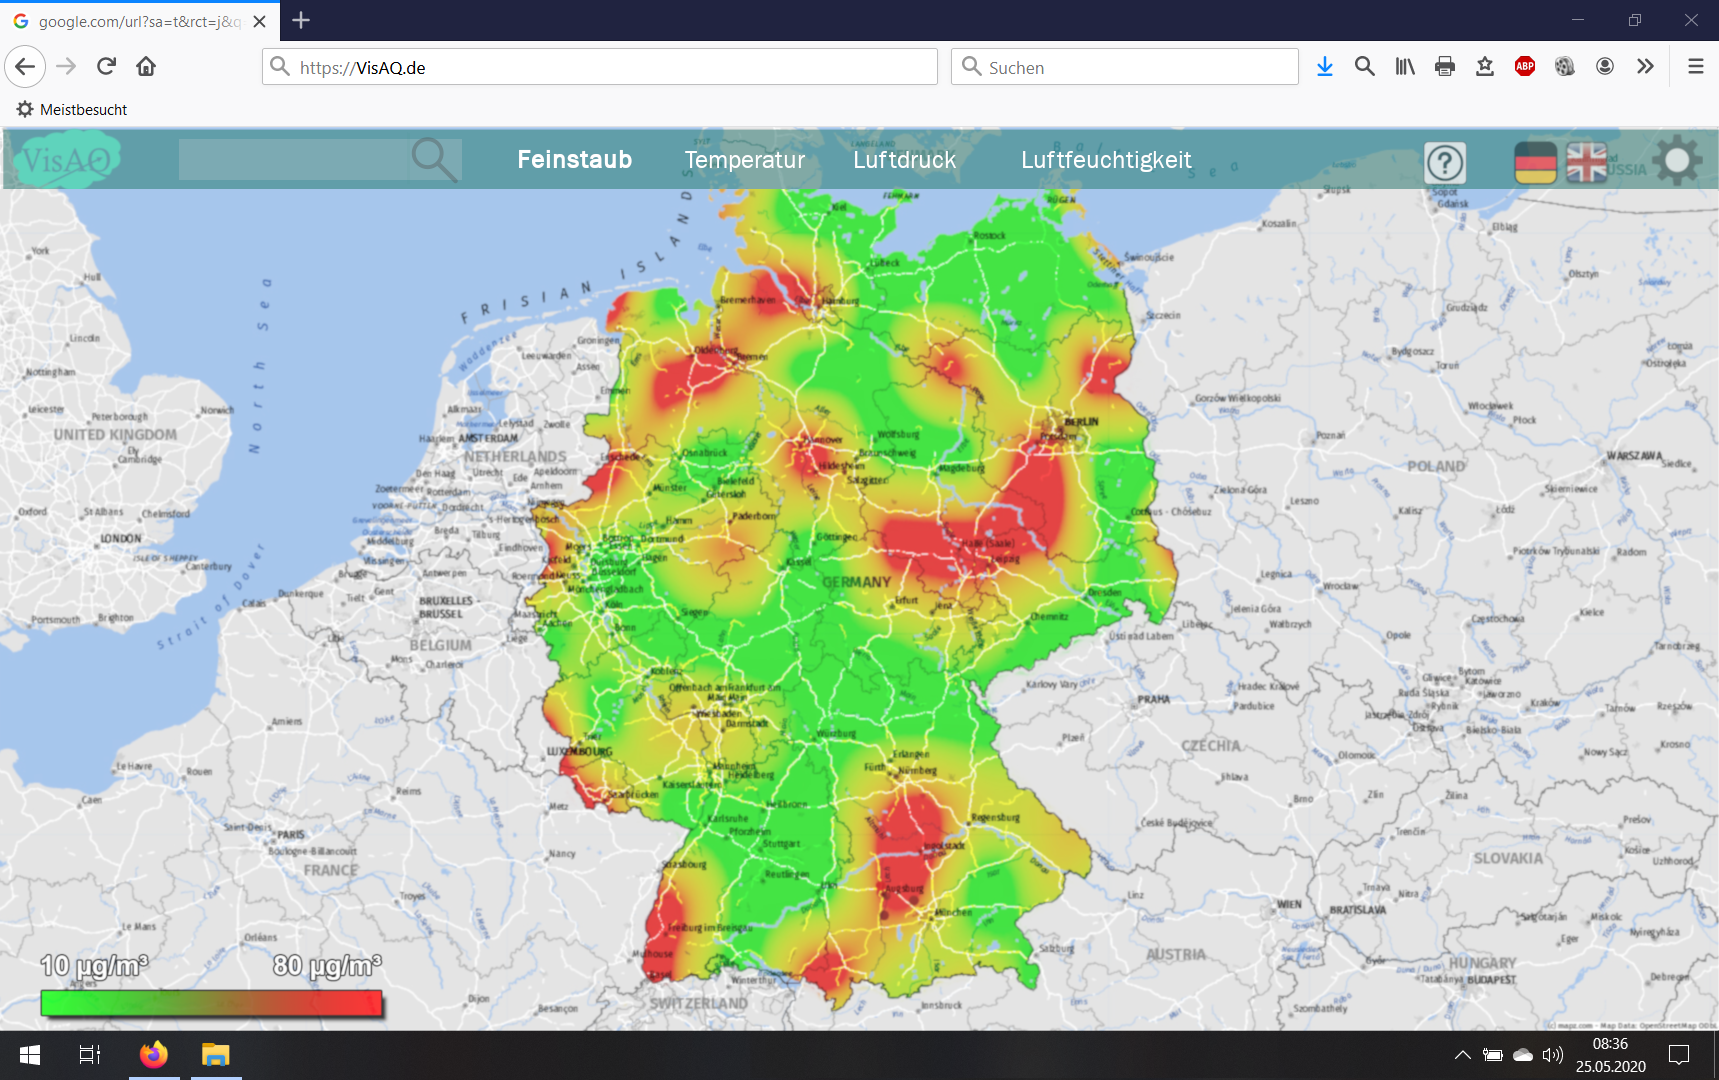
\includegraphics[width=0.9\textwidth]{media/Startseite}\captionof{figure}{Startseite} 

	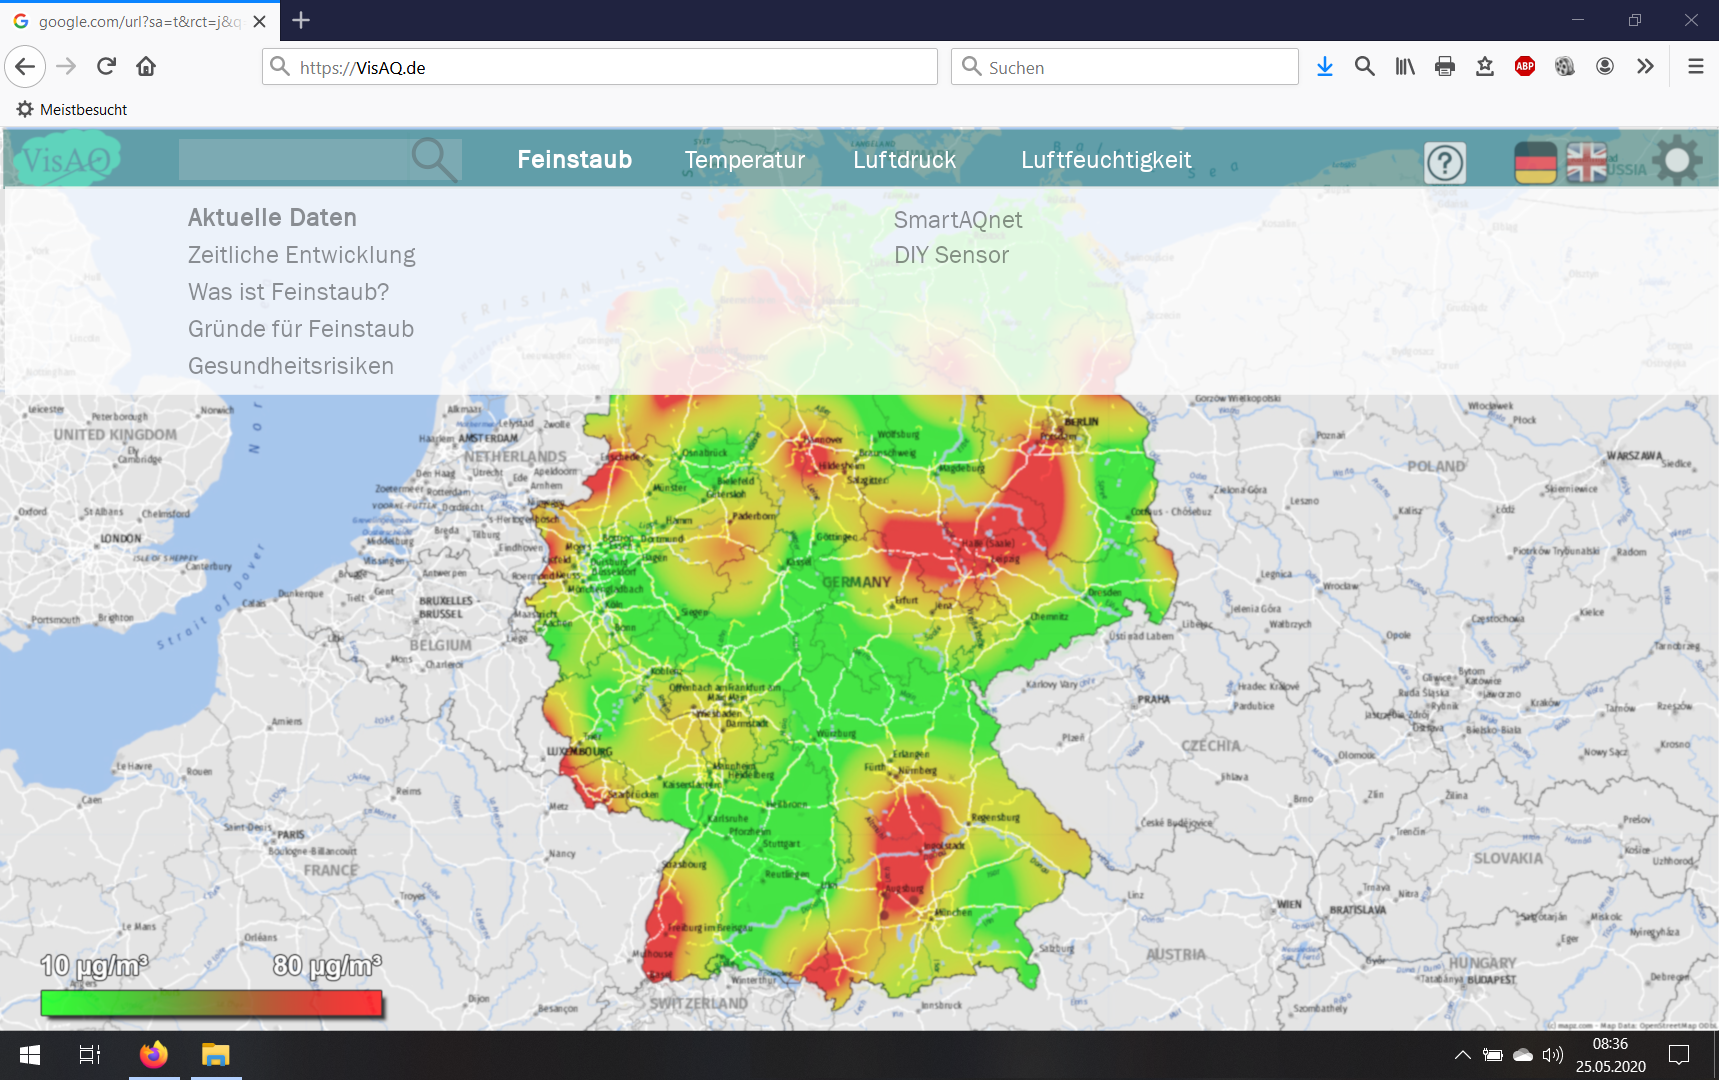
\includegraphics[width=0.9\textwidth]{media/Menue}\captionof{figure}{Menü} 

\vspace{1cm}
	
	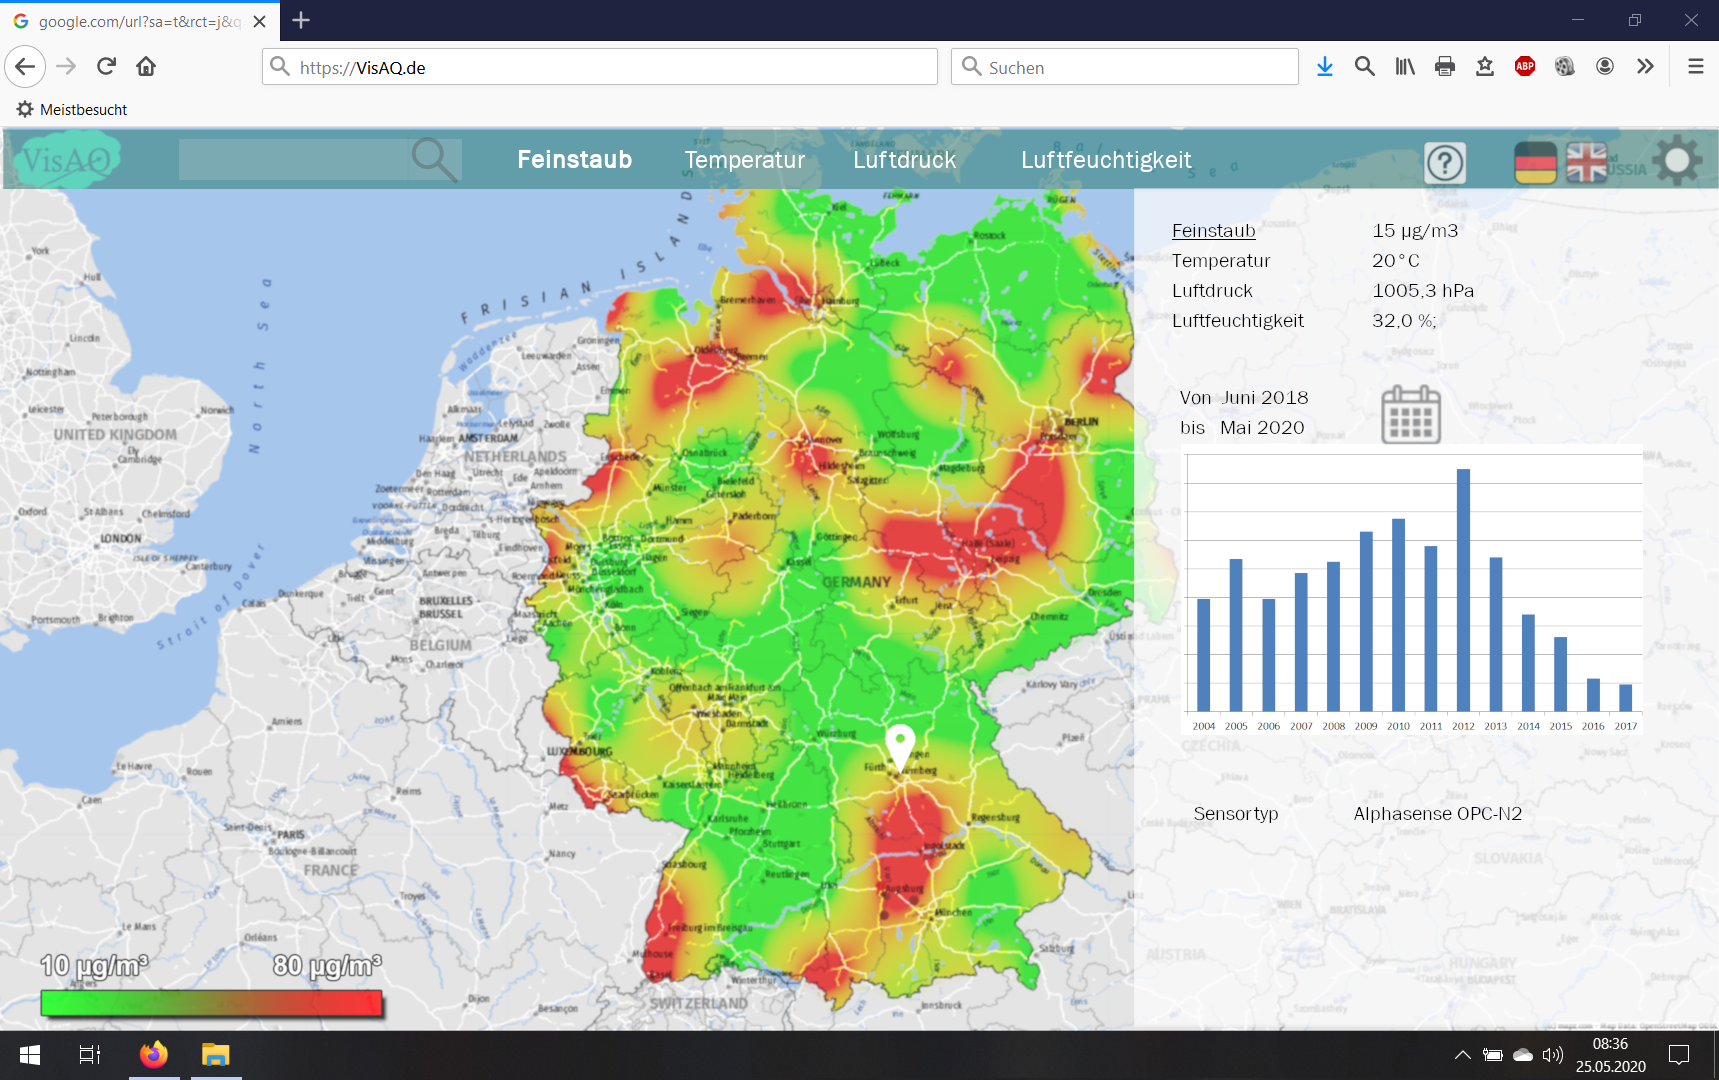
\includegraphics[width=0.9\textwidth]{media/Aktuelle-Daten}\captionof{figure}{Aktuelle Daten} 

	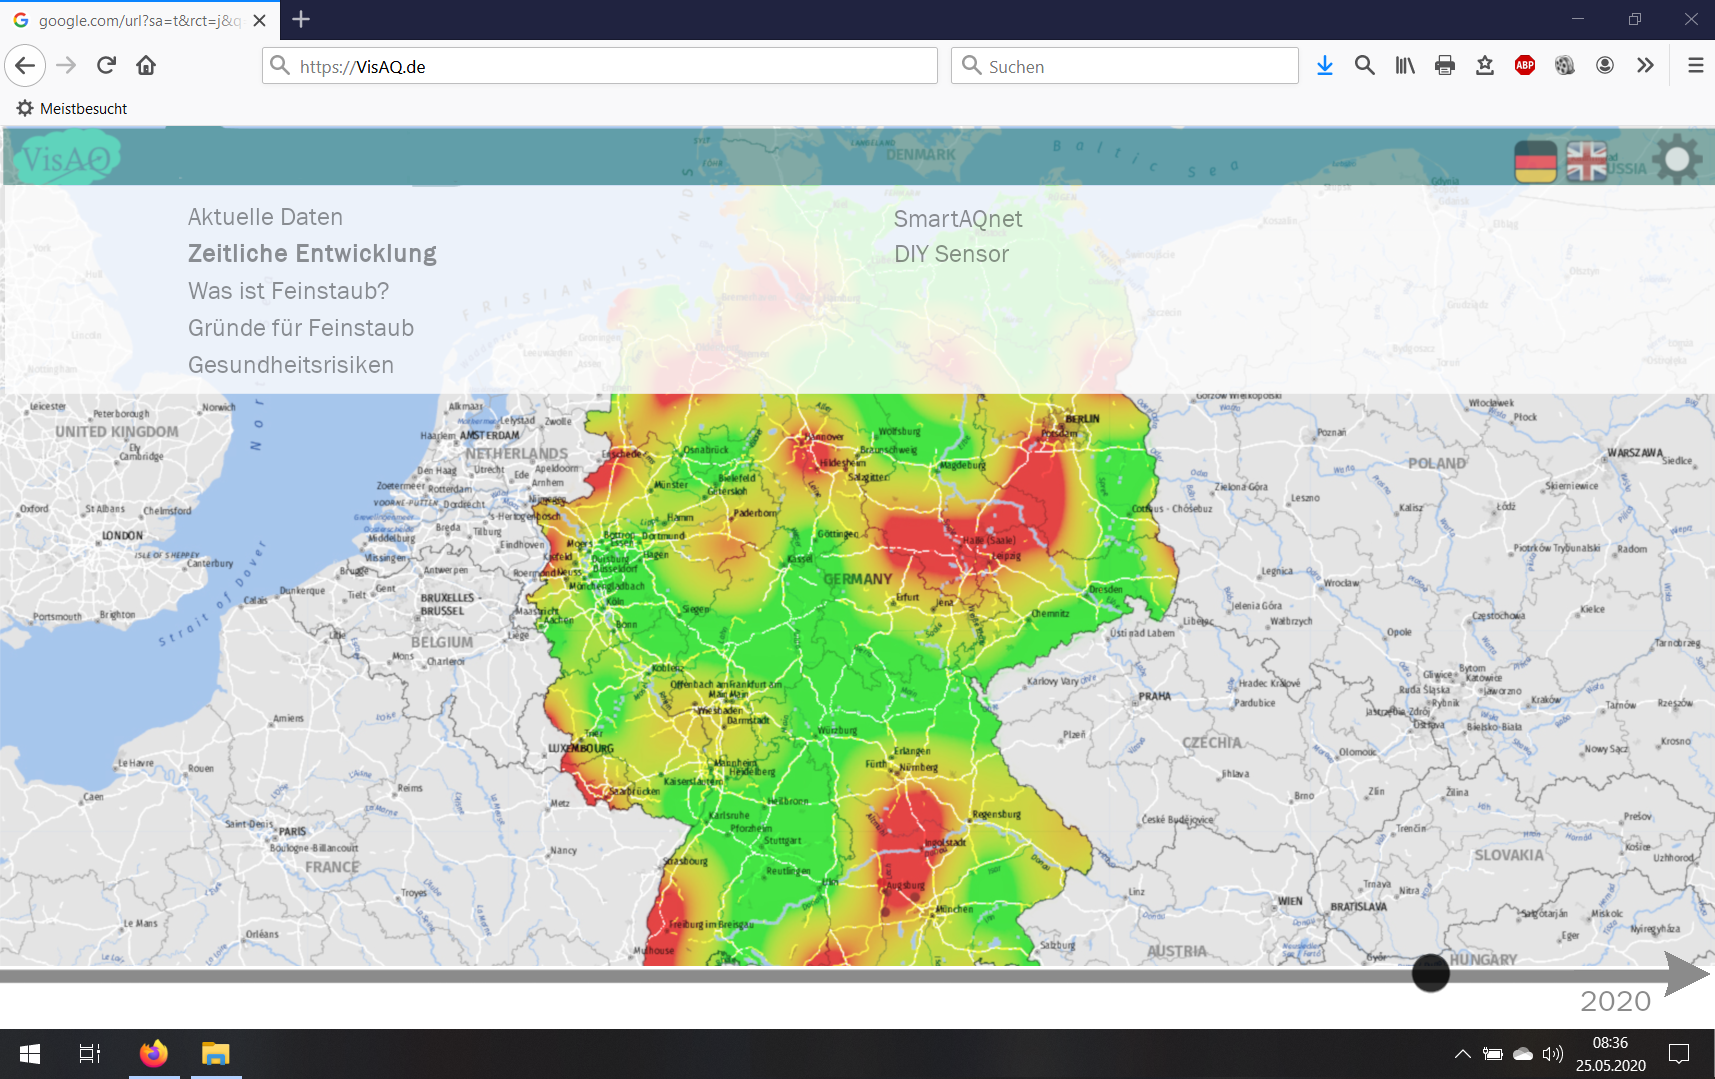
\includegraphics[width=0.9\textwidth]{media/Zeitliche-Entwicklung}\captionof{figure}{Zeitliche Entwicklung} 

\vspace{1cm}
	
	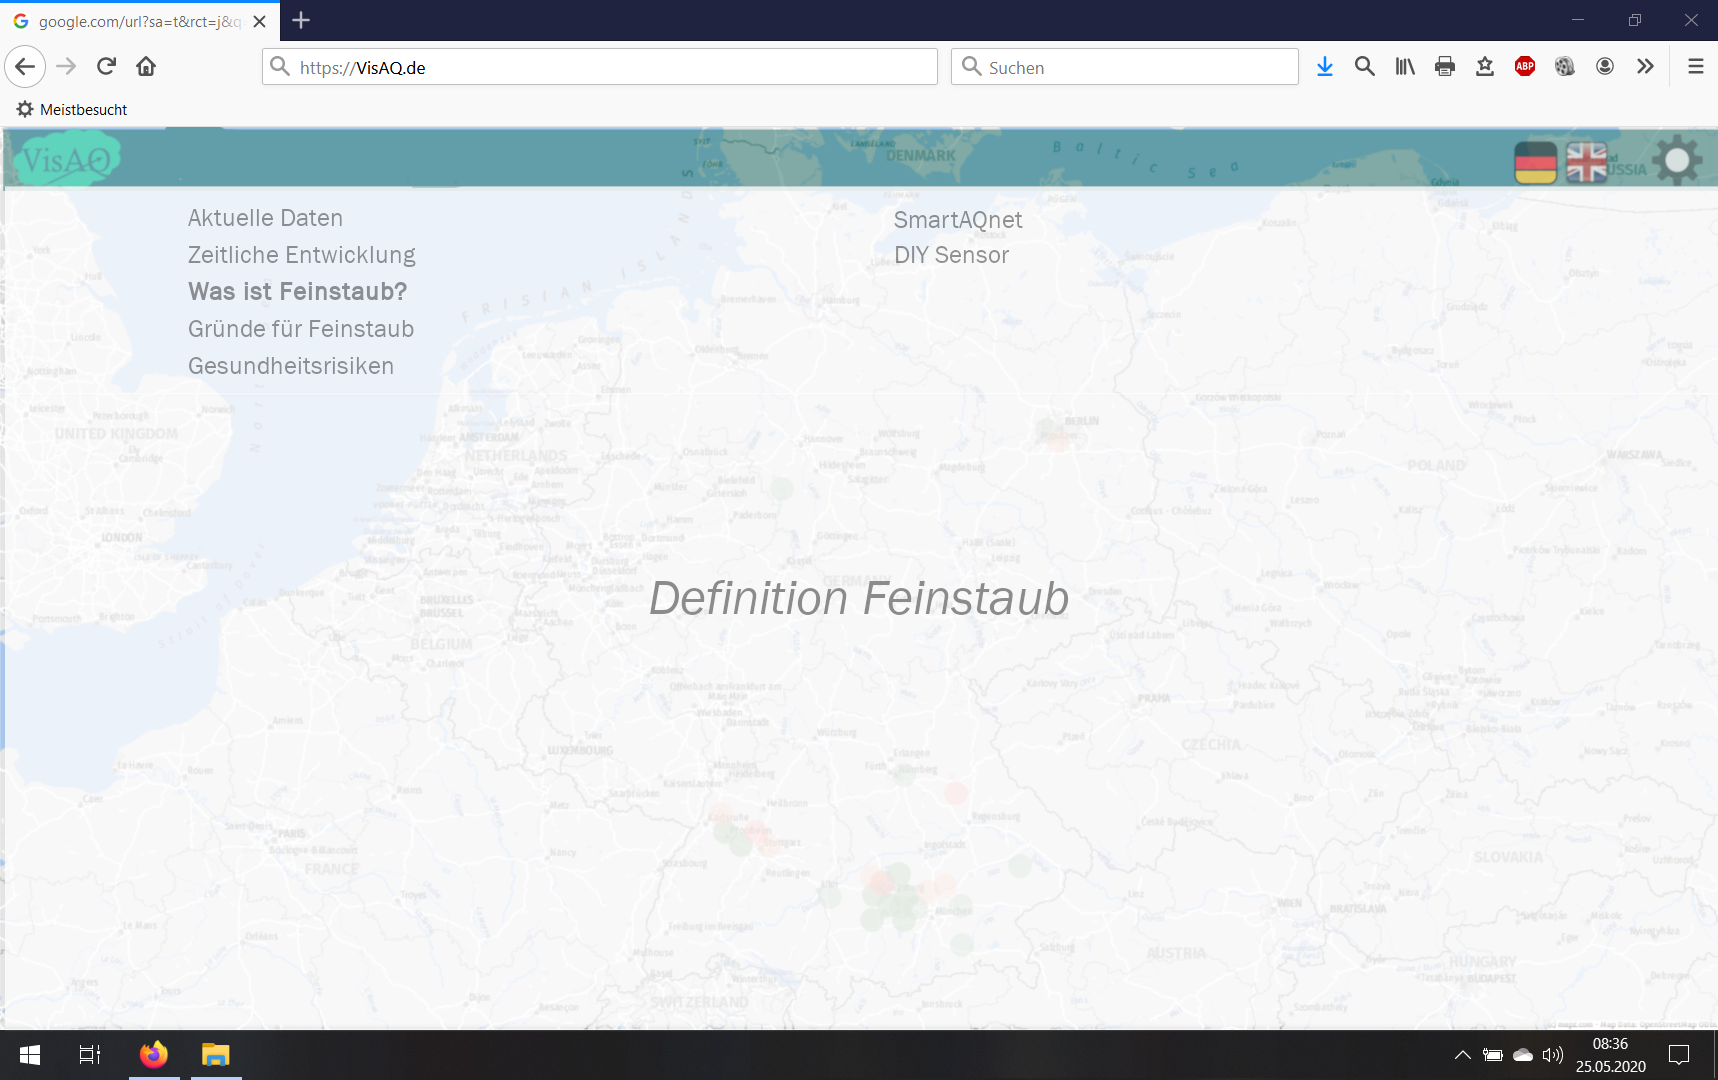
\includegraphics[width=0.9\textwidth]{media/Definition-von-Feinstaub}\captionof{figure}{Definition von Feinstaub} 
	
	
	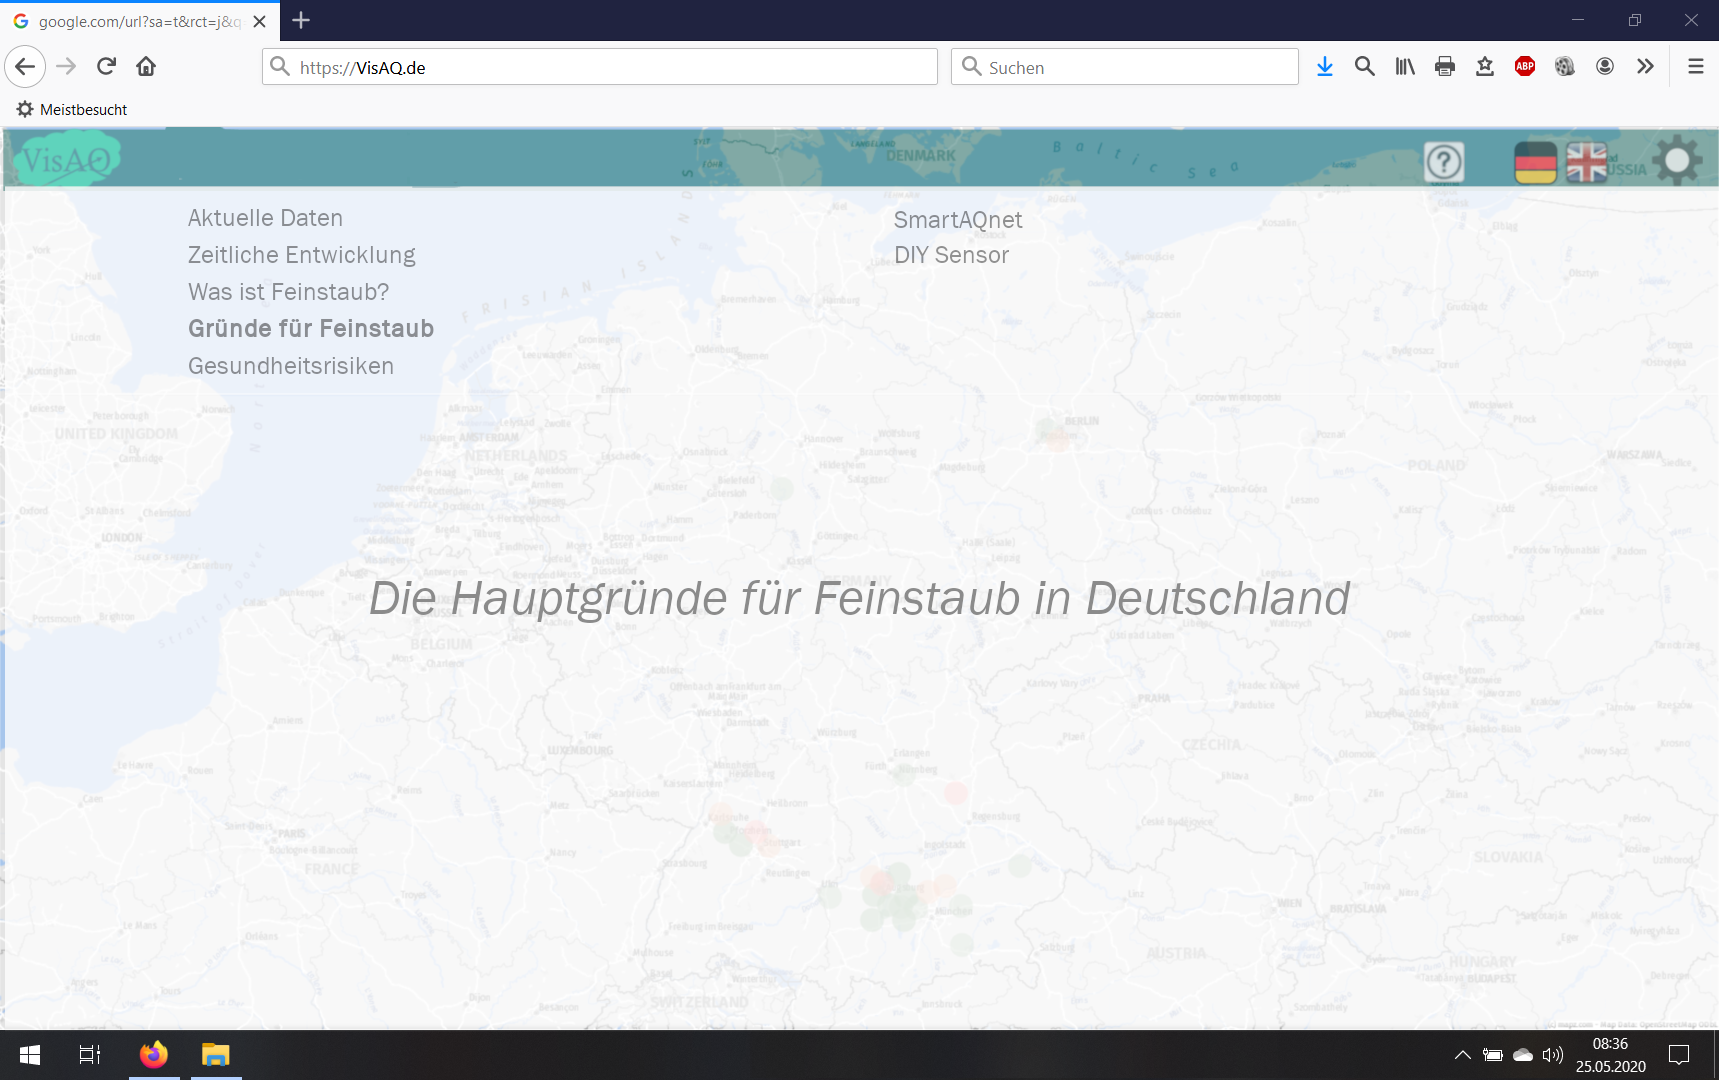
\includegraphics[width=0.9\textwidth]{media/Gruende-Feinstaub}\captionof{figure}{Hauptgründe für Feinstaub in Deutschland} 
	
\vspace{1cm}	
	
	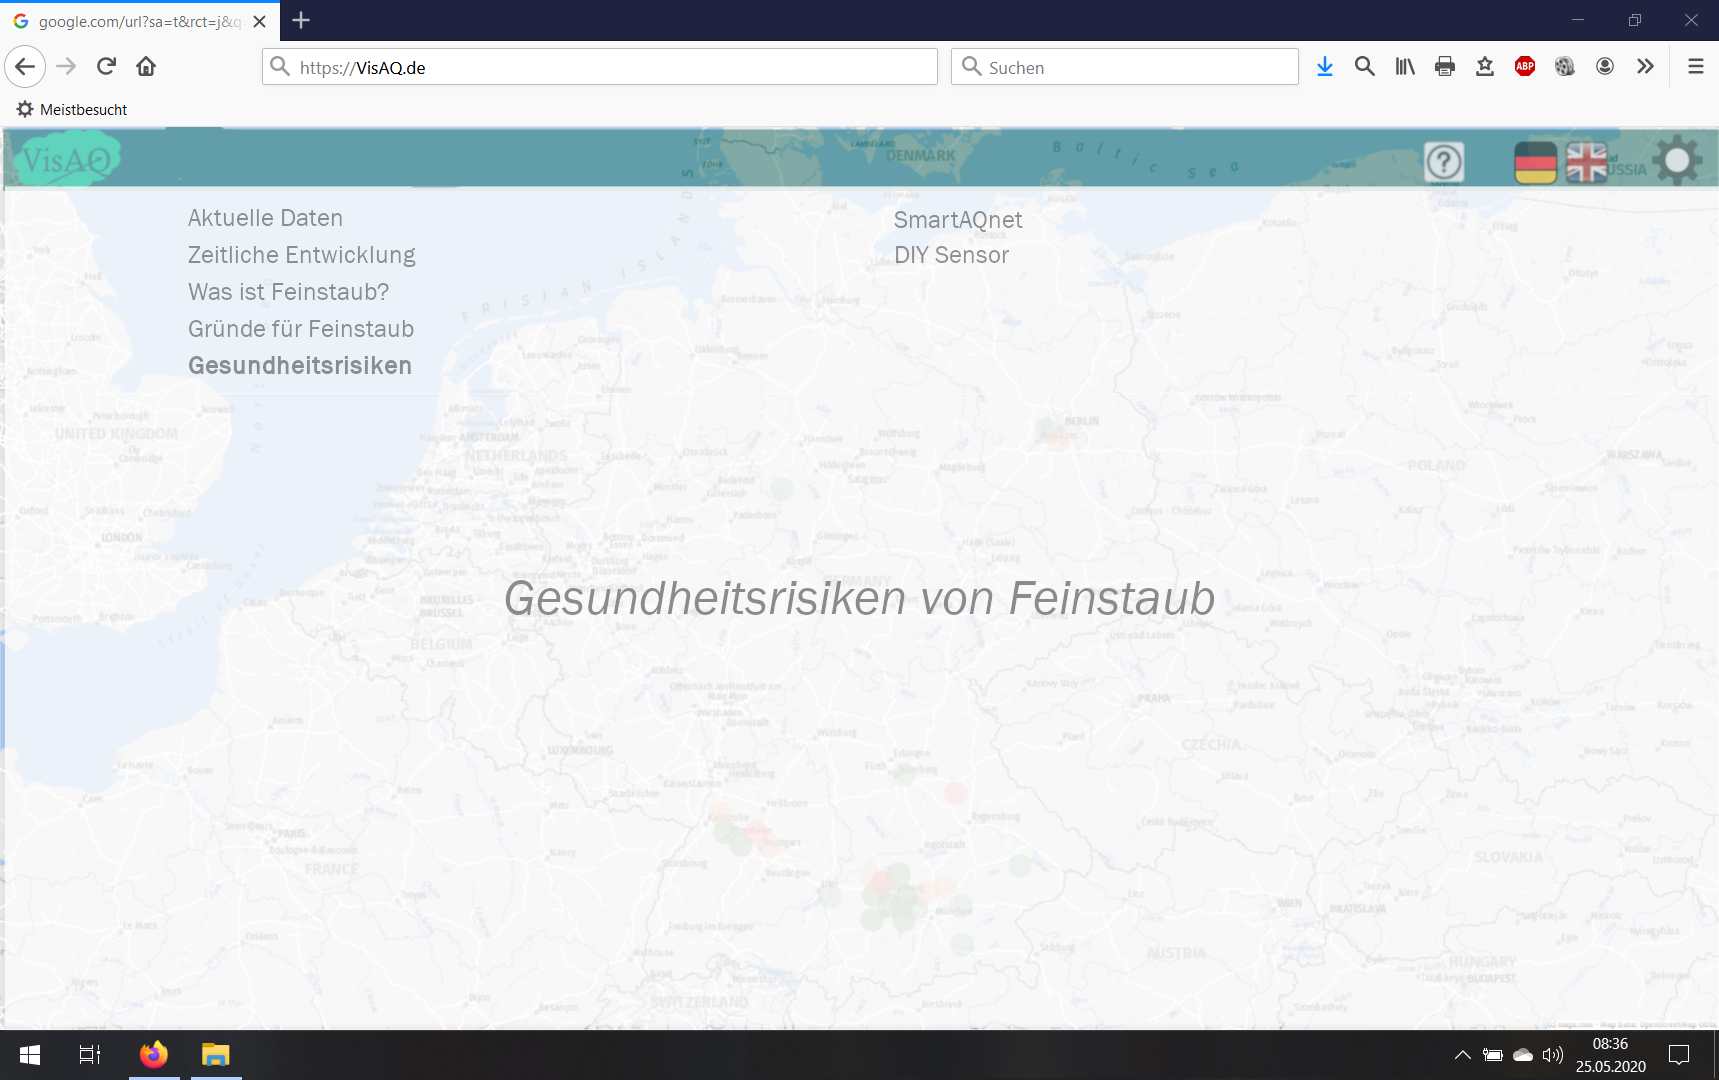
\includegraphics[width=0.9\textwidth]{media/Gesundheitsrisiken}\captionof{figure}{Gesundheitsrisiken von Feinstaub} 
	
	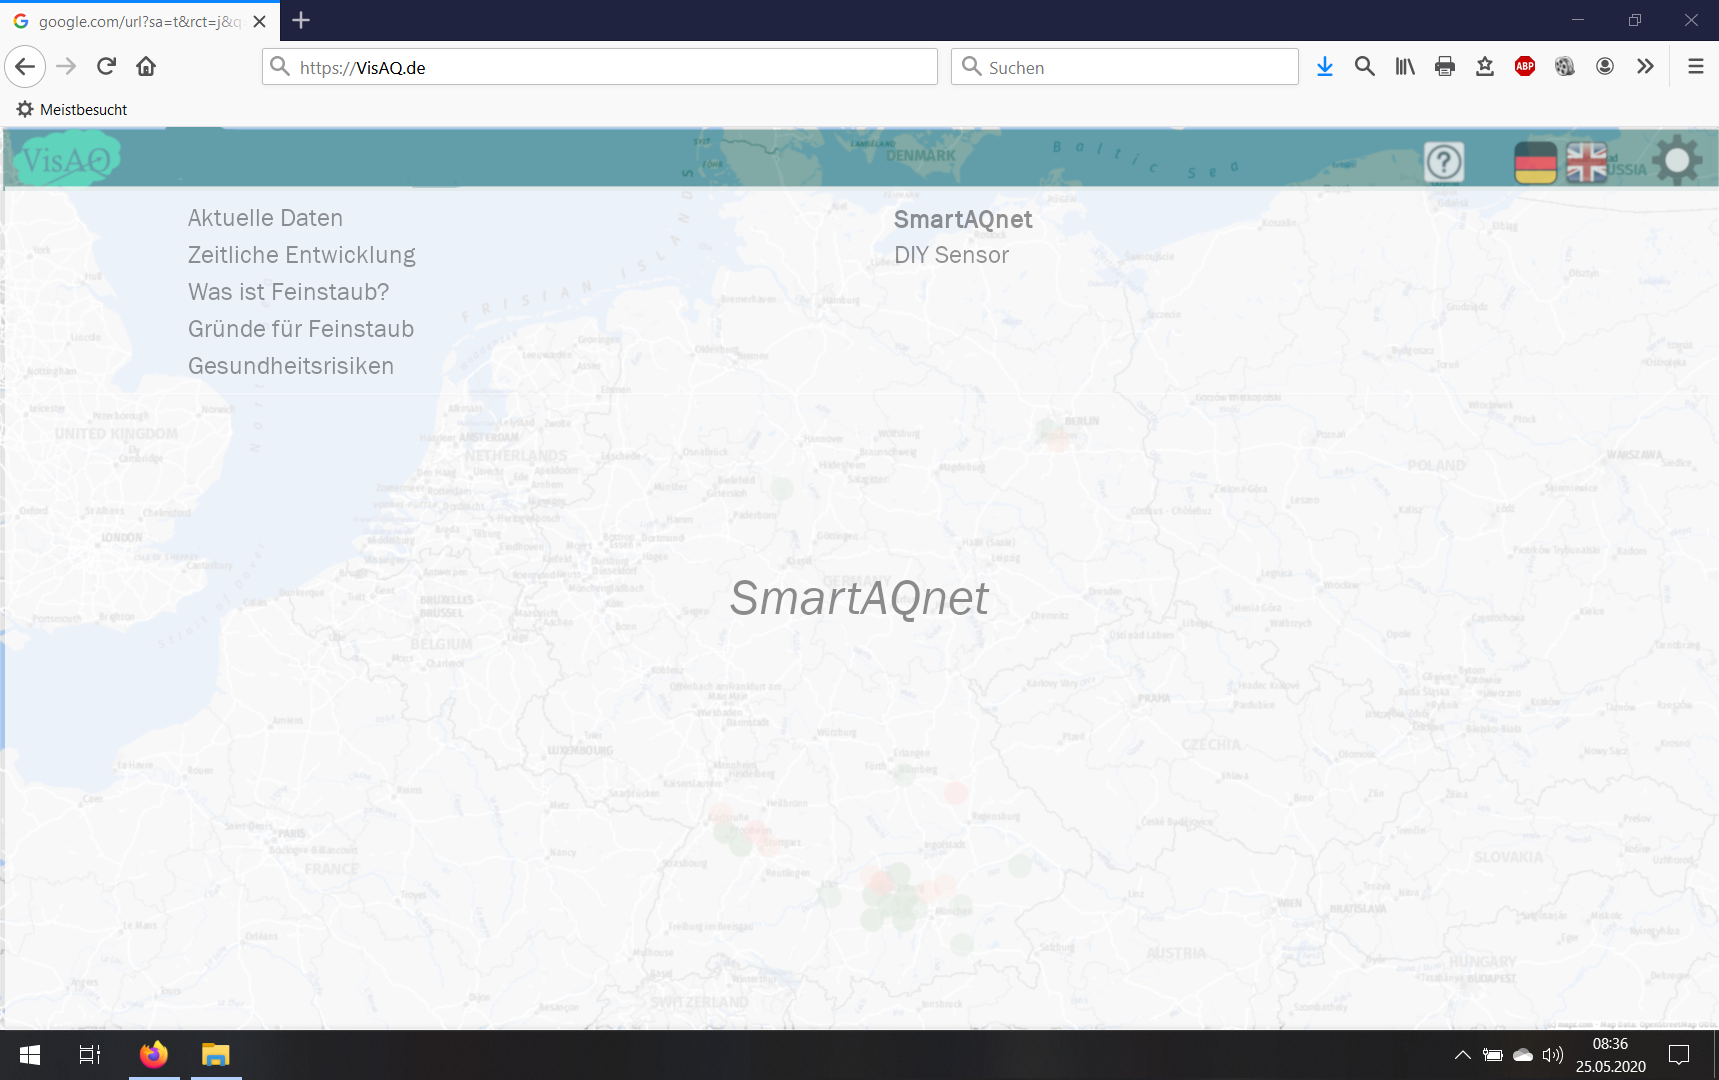
\includegraphics[width=0.9\textwidth]{media/SmartAQnet}\captionof{figure}{\gls{SmartAQnet}}

\vspace{1cm}
	
	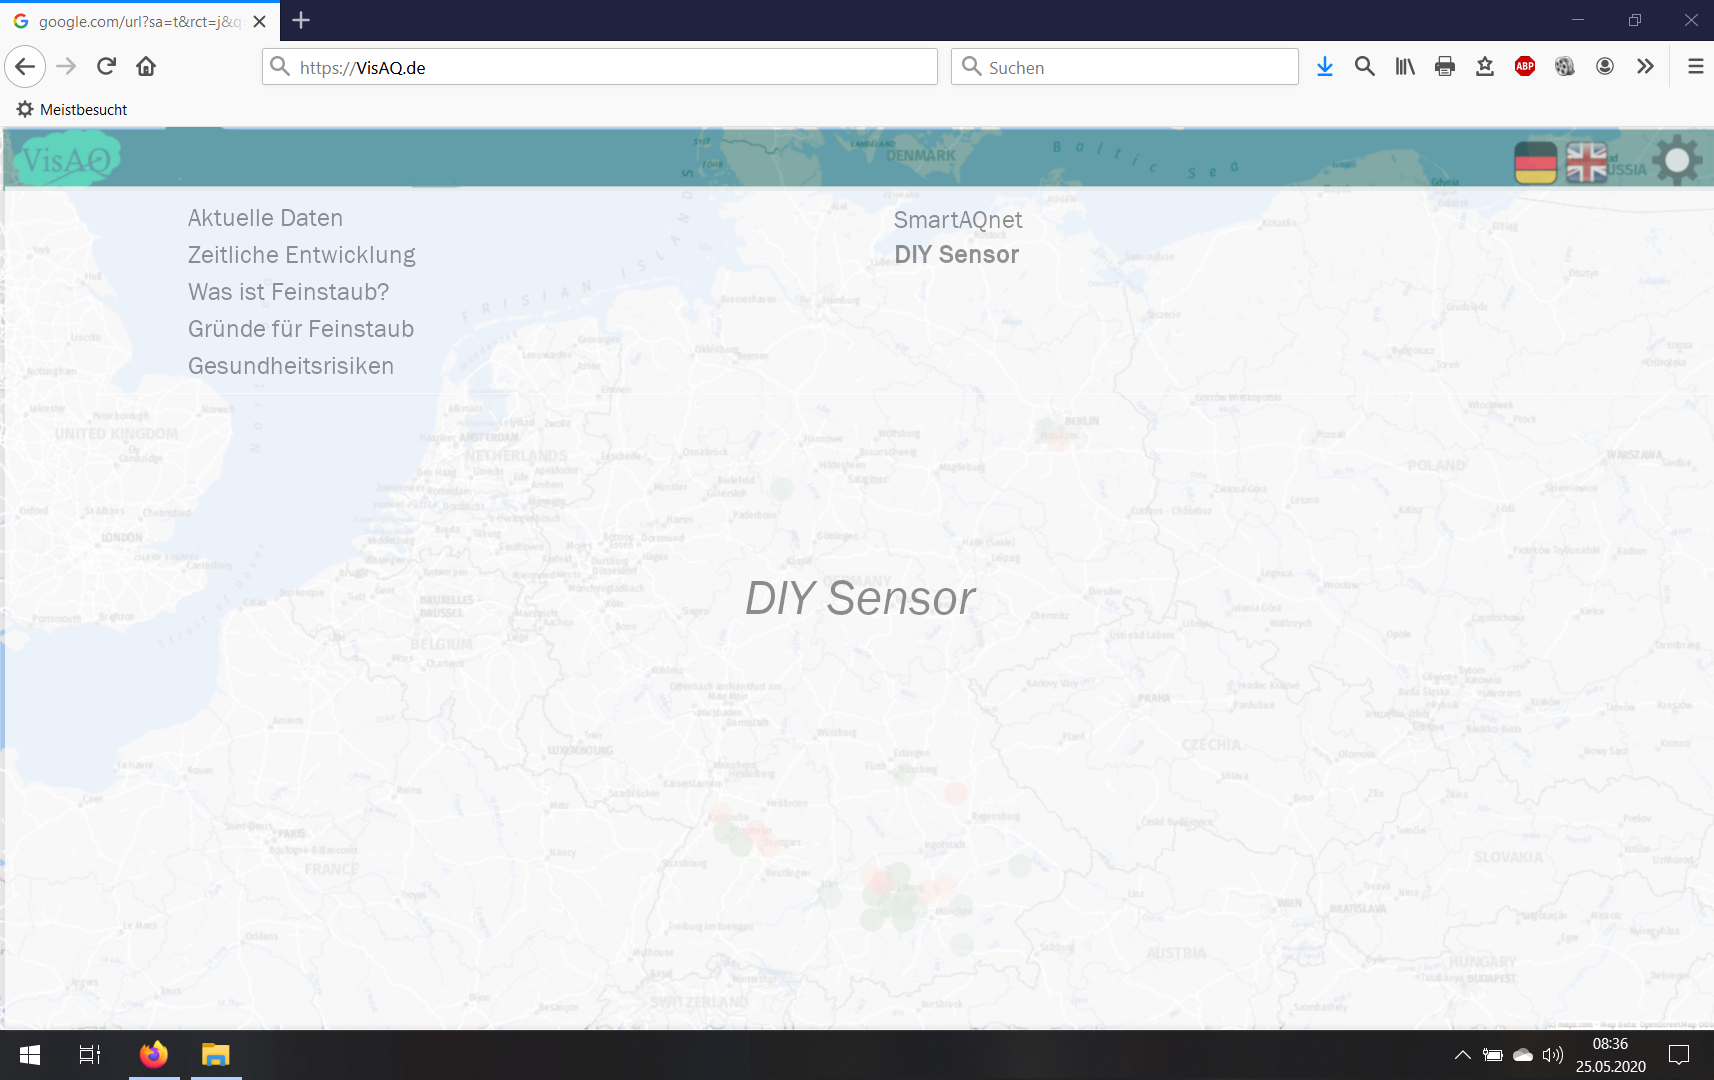
\includegraphics[width=0.9\textwidth]{media/DIY}\captionof{figure}{Verlinkung zu einer Bauanleitung für einen \gls{DIY}-\gls{Sensor}} 
\end{center}

\subsection{Screenshots Mobile Version}

\begin{figure}[H]
    \begin{subfigure}[c]{0.5\textwidth}
        \centering        
        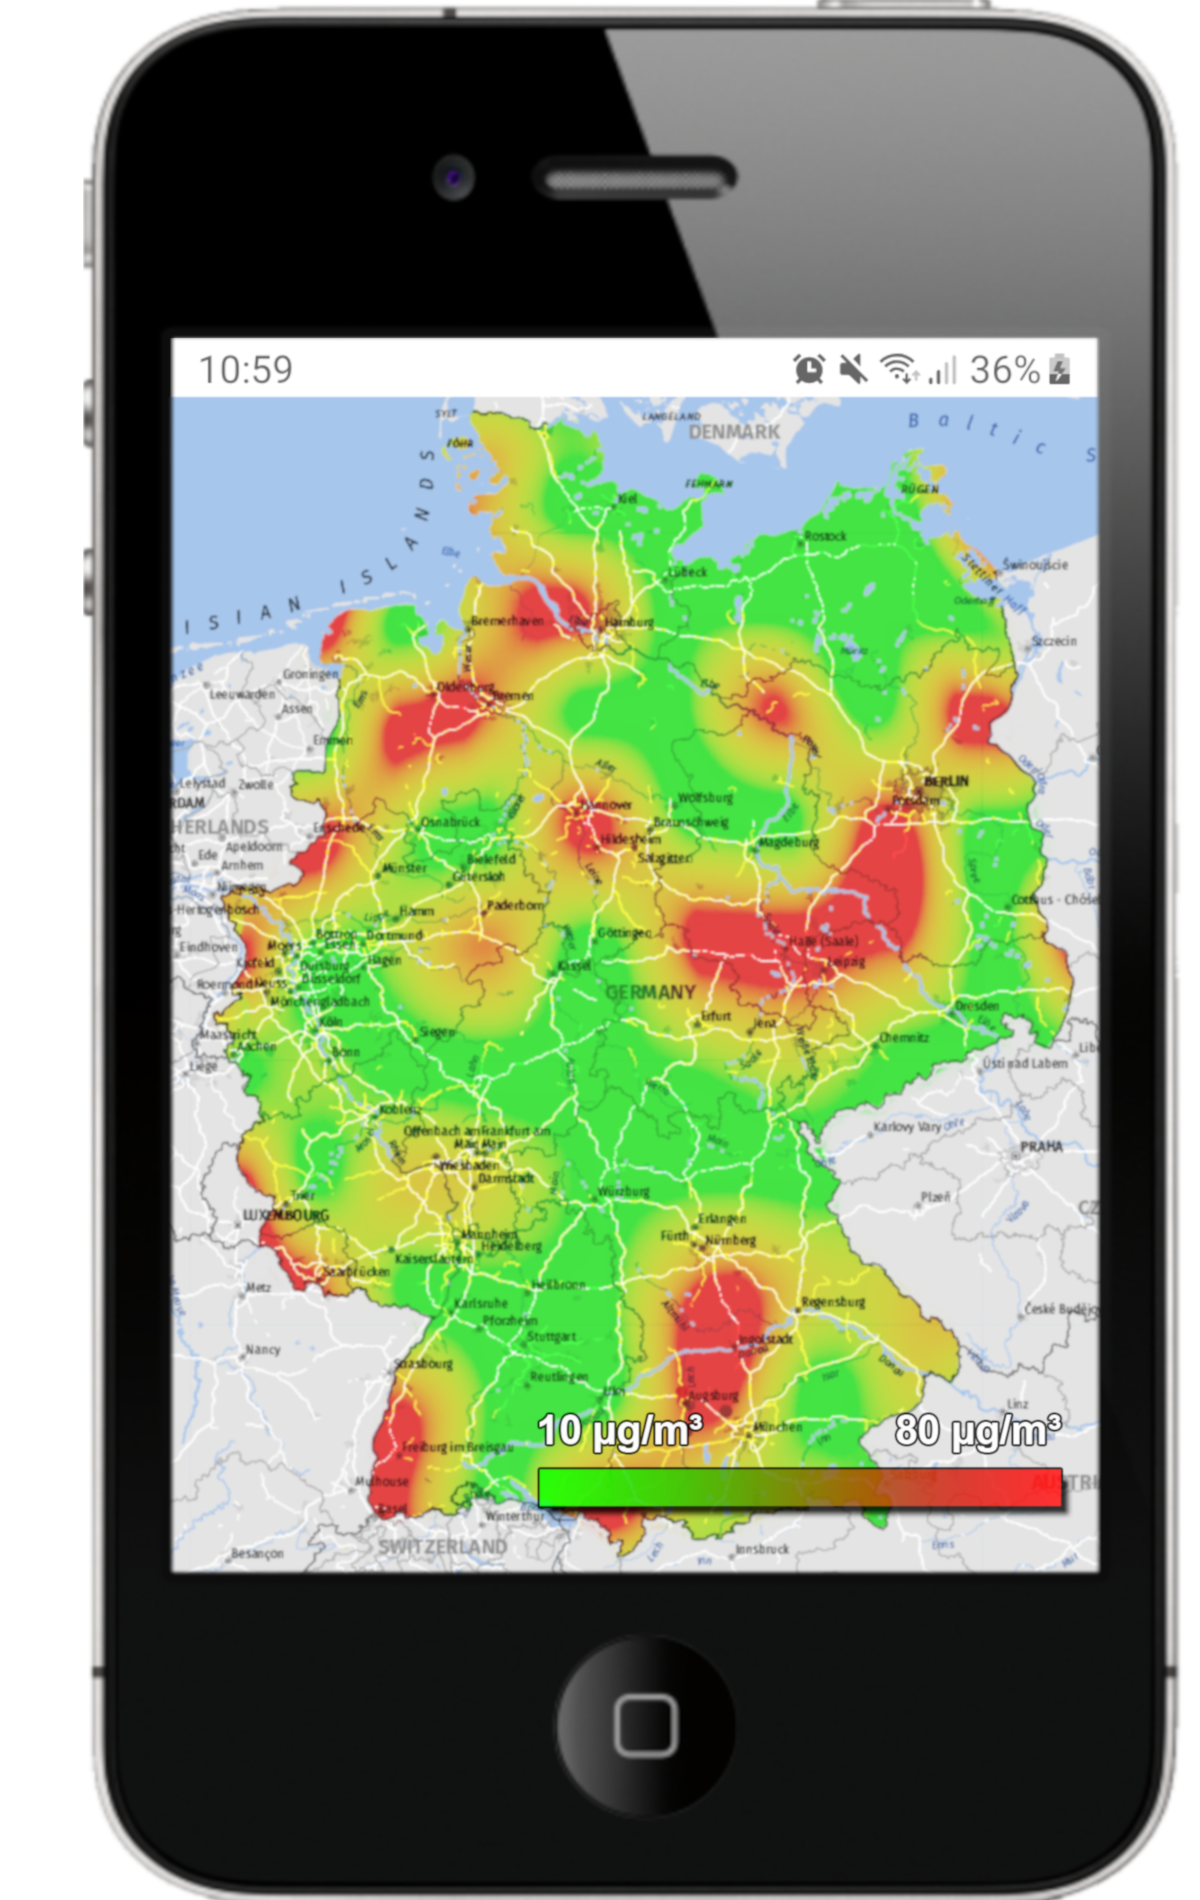
\includegraphics[scale=0.5]{media/Startseite-Mobile-Version}
        \subcaption{Startseite}
    \end{subfigure}
    \begin{subfigure}[c]{0.5\textwidth}
        \centering        
        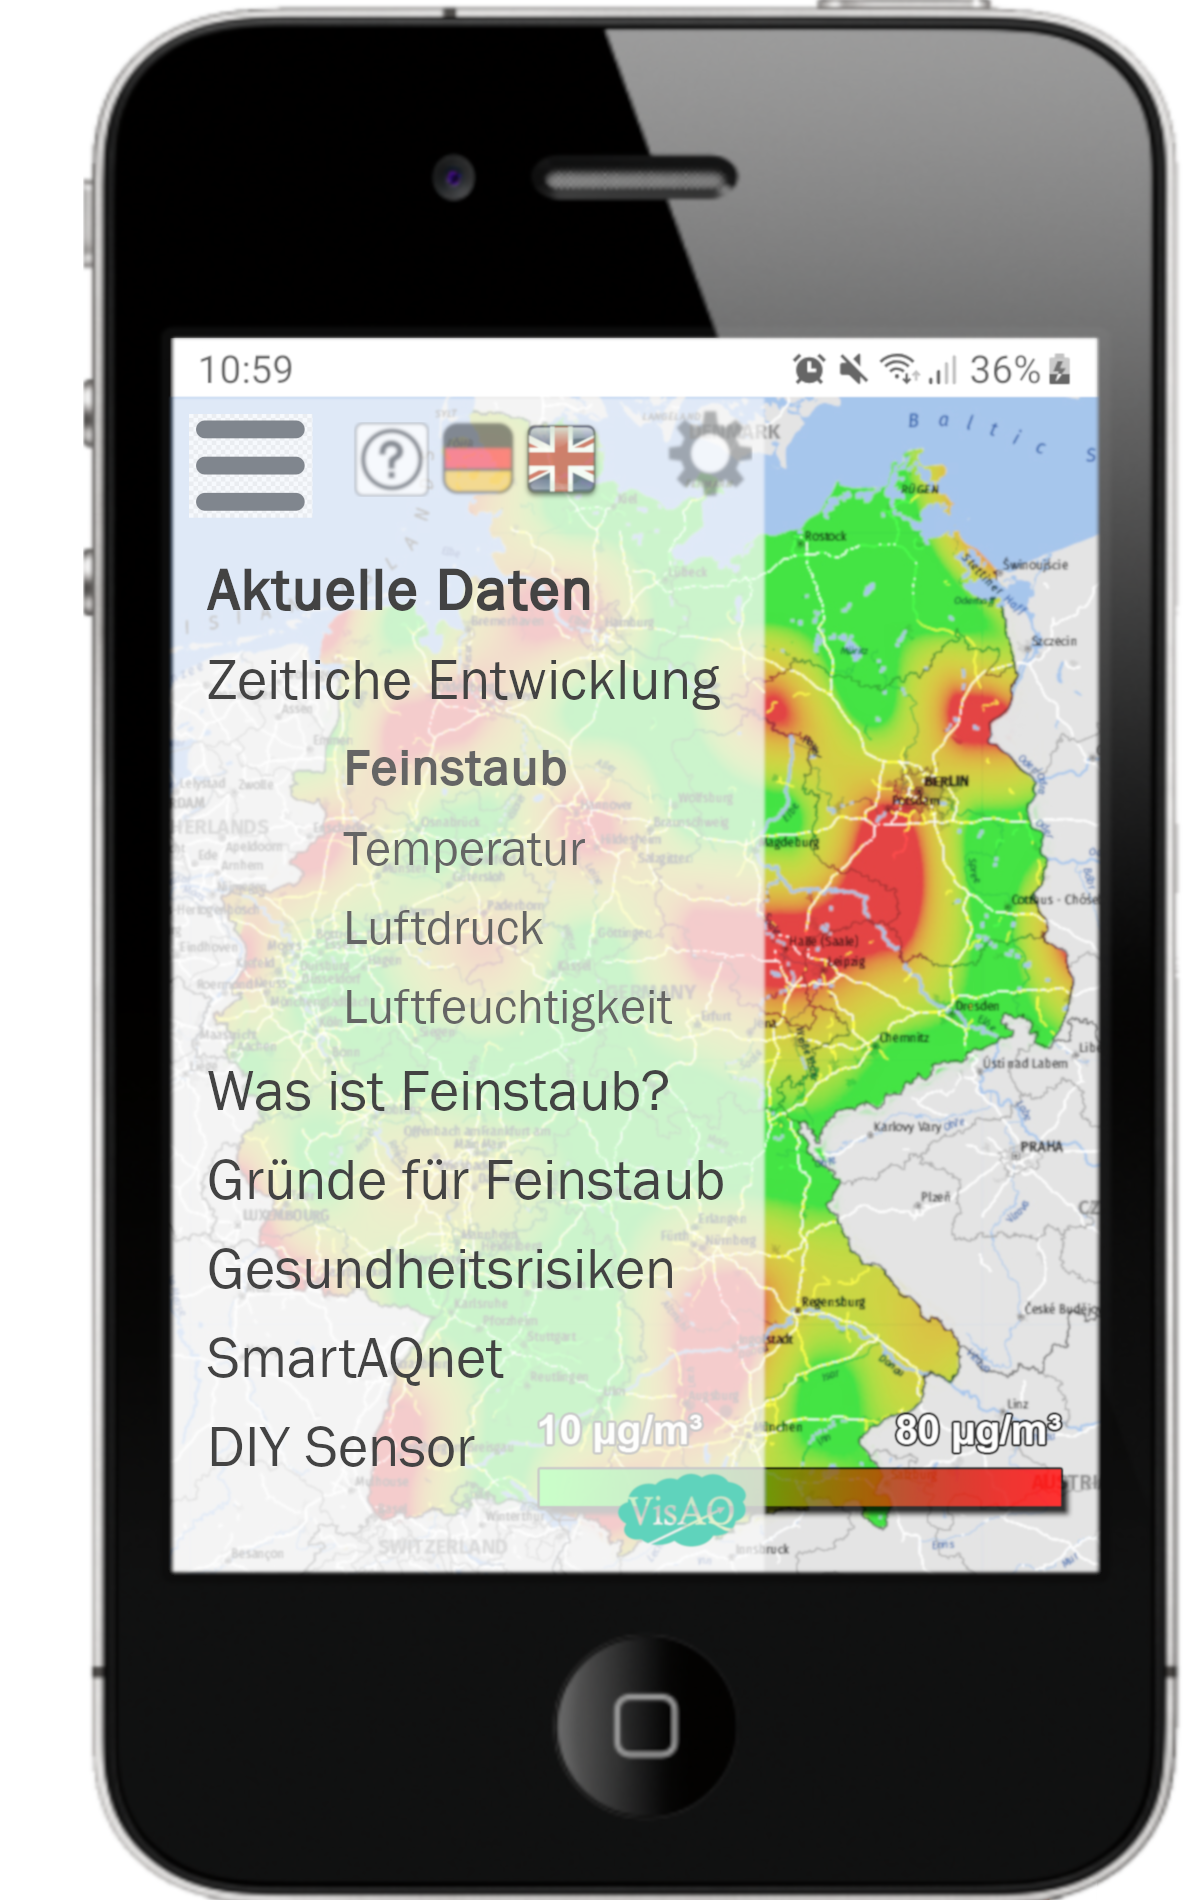
\includegraphics[scale=0.5]{media/Menue-Mobile-Version}
        \subcaption{Menü}
    \end{subfigure}
\end{figure}

\begin{center}
    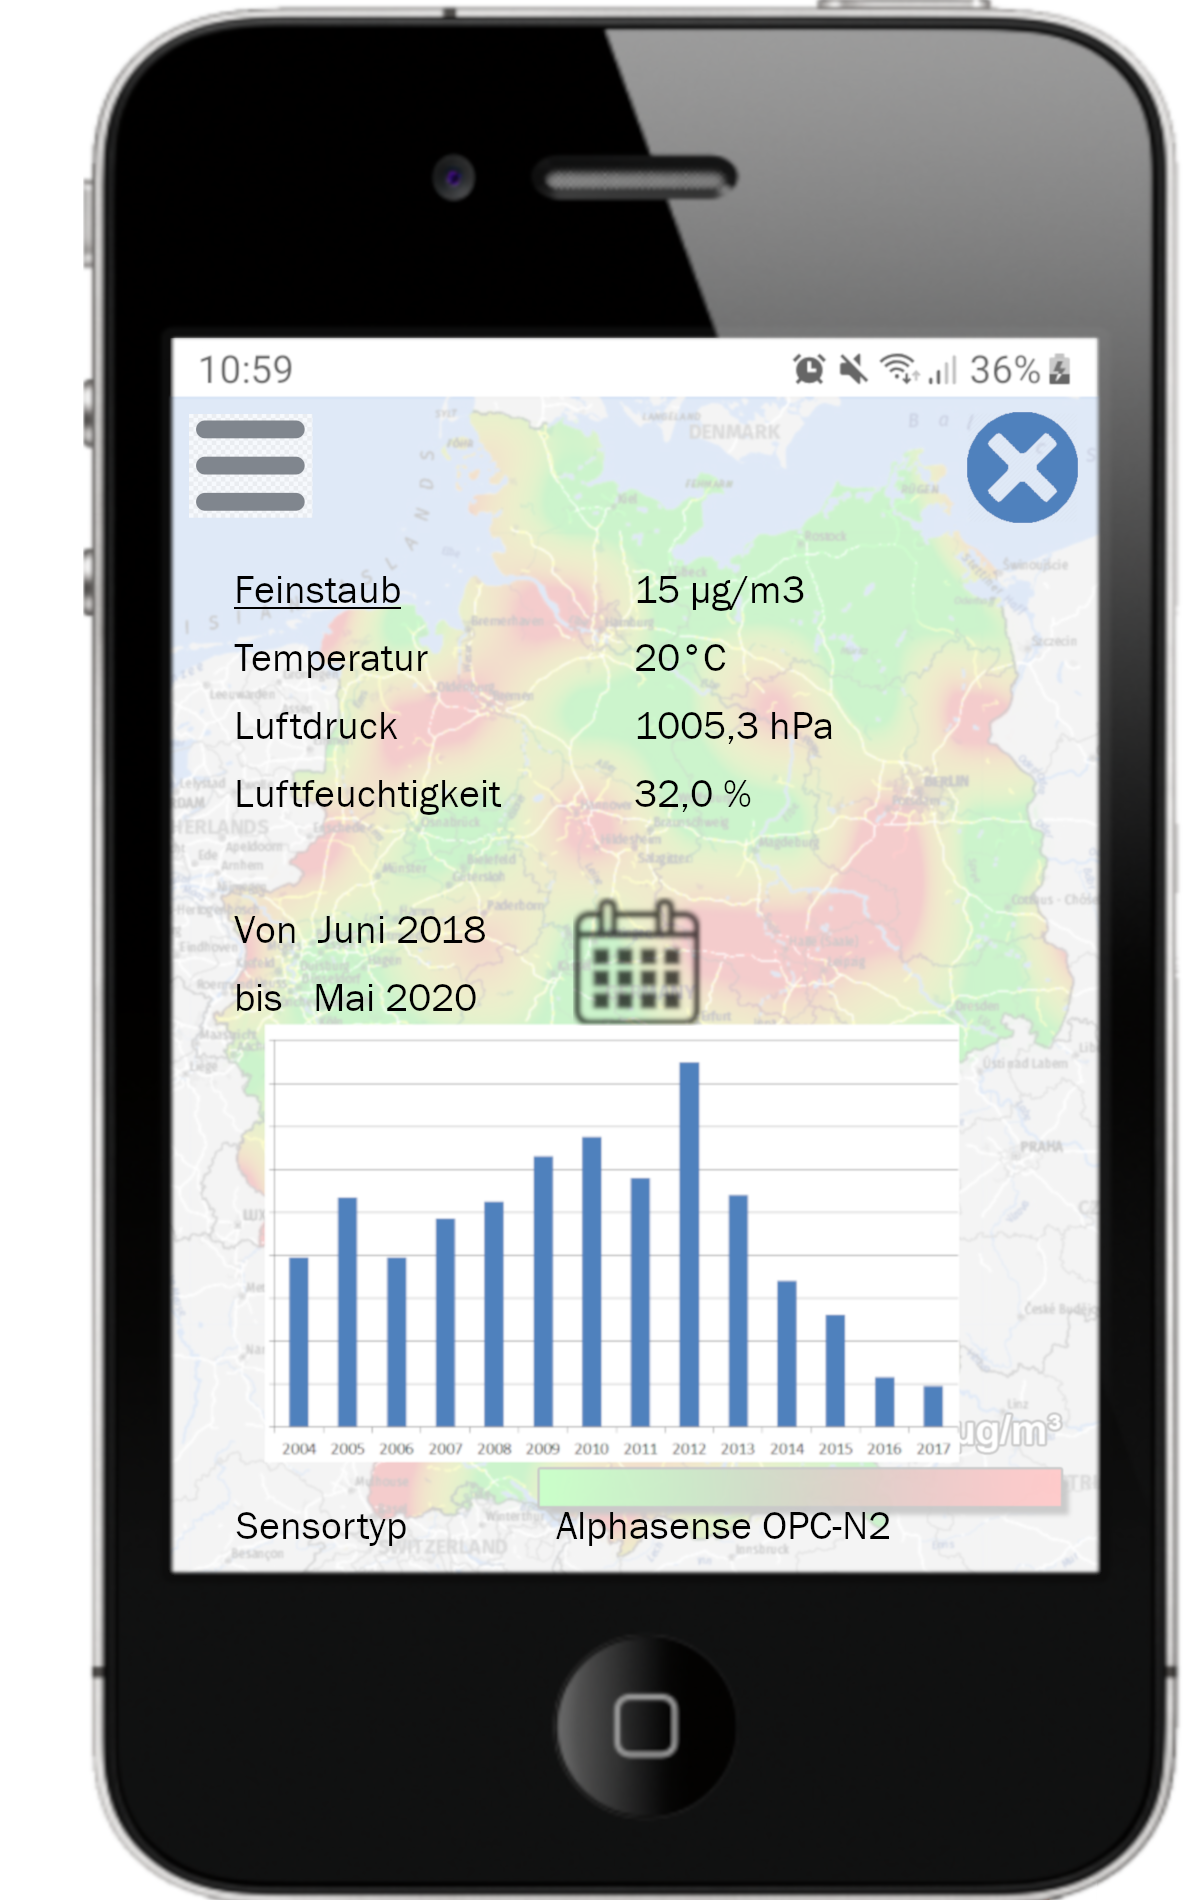
\includegraphics[scale=0.5]{media/AktuelleDaten-Mobile-Version}   
    \captionof{figure}{Aktuelle Daten} 
\end{center}

\textbf{Anmerkung:}
Es gilt zu beachten, dass die beschriebene Benutzeroberfläche in \autoref{Struktur Frontend} und \autoref{Screenshots} nur eine erste Annäherung an das Endprodukt ist. In der endgültige Version sind eventuell Abweichungen in der Darstellung der Daten möglich, jedoch ist die hier gegebene Struktur maßgeblich.

\section{Tests und Qualitätssicherung}
\begin{frame}{Qualitätszielbestimmungen}
    \begin{itemize}
        \item Durchschnittlich weniger als 1 Stunde Ausfall im Monat
        \item Stabilität unabhängig von der Stabilität der Datenbank
        \item Von Laien bedienbar
        \item Anschauliche für den Nutzer verständliche Visualisierung
        \item Keine Kopplung an bestimmten Webserver
        \item Bei Ausfall kein Datenverlust
    \end{itemize}
\end{frame}

\begin{frame}{Tests}
    
\end{frame}
\section{}
\questionframe
\lastframe
\end{document}